\documentclass[final]{article}
\usepackage[utf8]{inputenc}
\usepackage{nips_2017}
\usepackage{graphicx}
\usepackage{natbib}
\usepackage{booktabs}
\usepackage{float}
\bibliographystyle{apalike}

%\bibliographystyle{unsrt} % Use for unsorted references 

\bibliographystyle{plainnat} % use this to have URLs listed in References

% Title Page

\begin{abstract}

We seek to better understand the foregone gains of Medicaid expansion by estimating the effect of Medicaid expansion among states that did not expand Medicaid in 2014. Because downstream effects of Medicaid expansion are primarily mediated through increasing insurance coverage, understanding whether this effect is different between expansion states and non-expansion states is a first-step to estimating differential downstream effects. Moreover, existing literature suggests that Medicaid take-up rates differs by political partisan composition; as a result we might believe that take-up rates would have been lower in states that did not expand Medicaid. Using data from the American Communities Survey (ACS), we use weighting approaches to reweight longitudinal covariates from expansion regions to balance the covariate distribution from treated regions to match the control regions. Our results provide evidence both that the ETU is lower than existing estimates of the ETT, and that this differential is driven primarily by factors associated with conservative governance. 

\end{abstract}

\newpage

\begin{document}

\maketitle

\section{Introduction}

The 2010 Affordable Care Act required states to expand their Medicaid programs by 2014 to offer coverage to all adults with incomes at least 138 percent of the federal poverty line (FPL). The Supreme Court ruled this requirement unconstitutional in 2012, allowing states to decide whether or not to expand Medicaid coverage. In 2014, twenty-six states and the District of Columbia expanded their Medicaid programs. \footnote{From 2015 through 2019 an additional ten states elected to expanded their Medicaid programs.} This first wave of expansions in 2014 created a so-called ``natural experiment", enabling researchers to examine the effects of Medicaid expansion by using expansion states as ``treated'' states, and non-expansion states as ``control'' states.\footnote{Due to heterogeneity in state Medicaid eligibility requirements prior to 2014, actual classifications in practice can be somewhat more complicated.} Hundreds of papers have been published over the last several years examining the effect of Medicaid expansion on myriad outcomes relating to healthcare and public health.

Our goal is to model the effect of 2014 Medicaid expansion on non-elderly adult uninsurance rates among non-expansion states. This would be uninteresting if all eligible individuals enrolled in Medicaid; however, because enrollment is not automatic, Medicaid take-up rates are lower than 100 percent and historically have varied across states (\cite{sommers2012understanding}). This variation in Medicaid take-up rates is partly a function of state discretion in administering programs: for example, program outreach, citizenship verification policies, and application process differ across states (\cite{courtemanche2017early}). 

Previous literature has only targeted the treatment effect on the treated (ETT). Existing estimates place the ETT between -3 and -6 percentage points; these estimates vary depending on the targeted sub-population of interest, the data used, and the modeling approach (see, eg, \cite{courtemanche2017early}, \cite{kaestner2017effects}, \cite{frean2017premium}). While it may be tempting to extrapolate these findings to estimate the ETU (see, eg, \cite{miller2019medicaid}), we believe this will lead to misleading inferences, given the heterogenous economic, demographic, and political characteristics of these groups of states.

We are especially concerned about how the political composition would drive differences between these effects because the decision to expand Medicaid in 2014 largely fell along partisan lines. Figure 1 plots each state's 2013 institutional ideology score by their Medicaid expansion status. Higher values of this score correspond to more liberal institutions. Non-expansion states are significantly more conservative than expansion states. Moreover, the 2014 Medicaid expansion, \cite{sommers2012understanding} found that a state's political ideology was associated with lower Medicaid enrollment take-up rates, even after controlling for a variety of correlated policies. If the differential take-up rates observed by \cite{sommers2012understanding} continue to hold post-expansion, we should expect treatment effects on non-expansion states to be lower than treatment effects on expansion states. 

\begin{figure}
    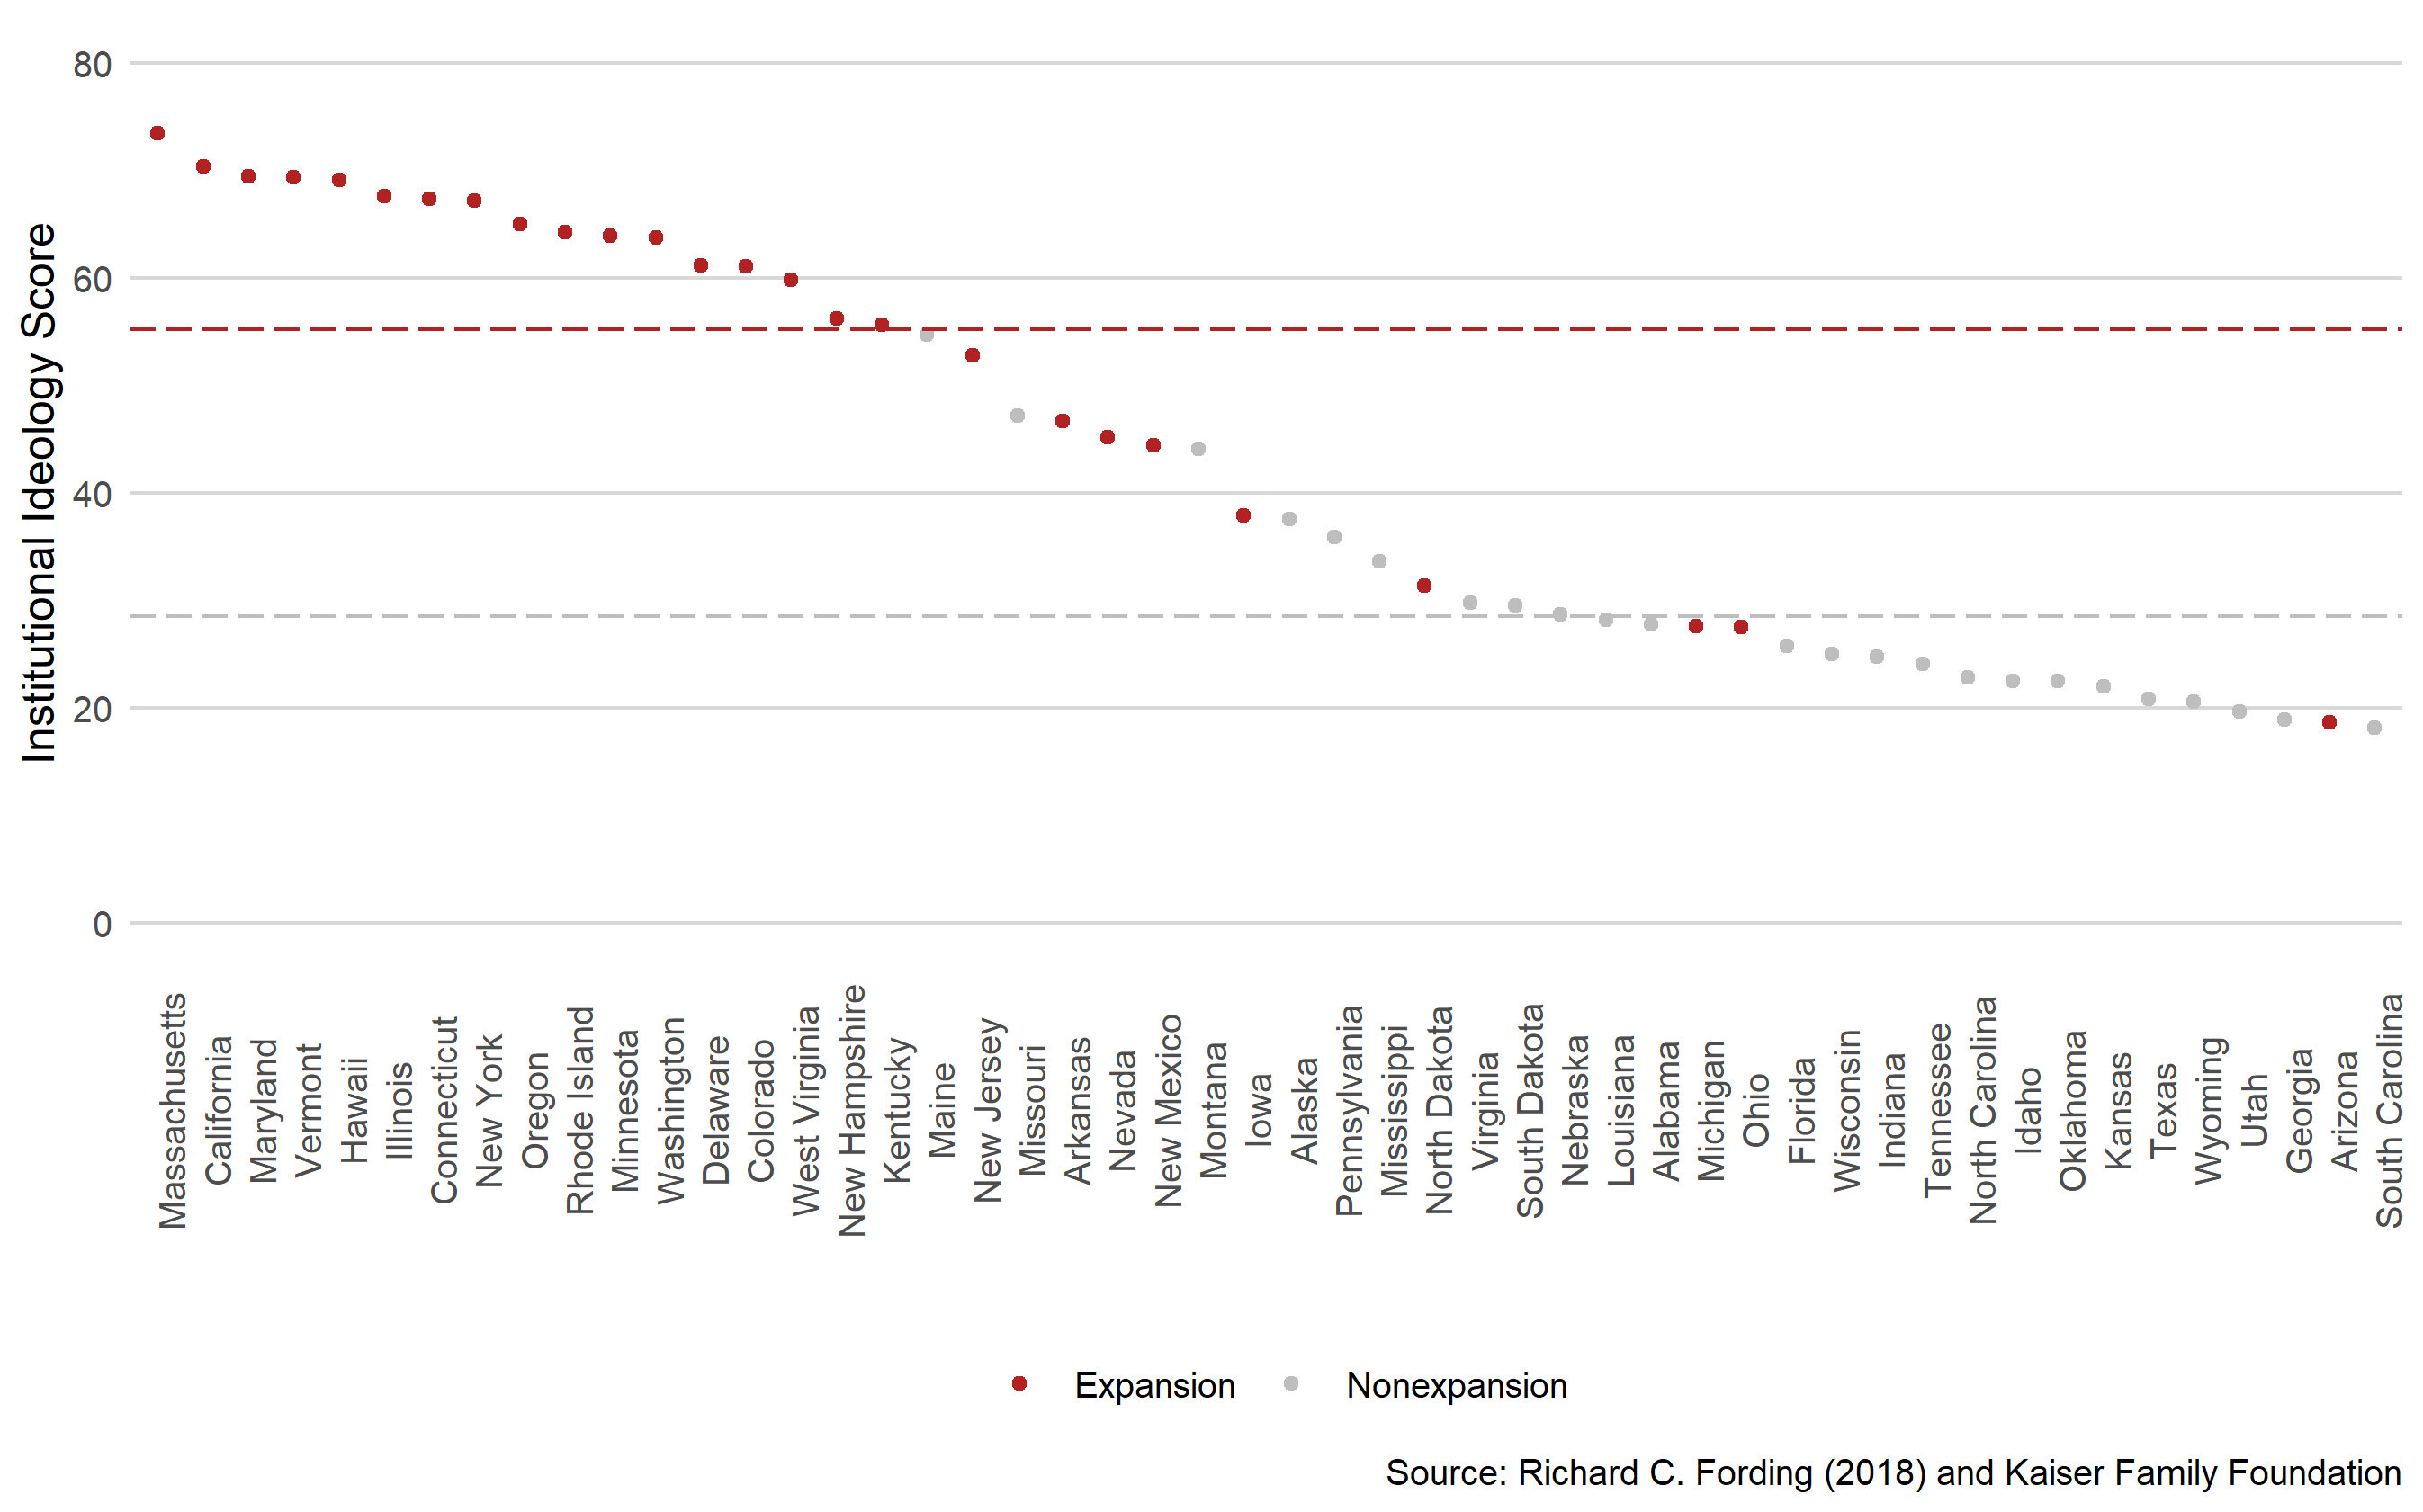
\includegraphics[scale=0.7]{political-expansion-plot.png}
    \caption{Political ideology and Medicaid expansion}
\end{figure}

Furthermore, given that the effects of Medicaid expansion are primarily mediated through insuring the previously uninsured, we can assume that if the ETU were closer to zero than the ETT, then further downstream effects that grow monotonically with the number of insured would also be attenuated. For example, Wherry and Miller use their estimate of the ETT to project that had all states expanded Medicaid in 2014, XXX deaths would have been avoided. If we believe that the ETT were lower than the ETU, we should expect this projection to be an overestimate. Directly estimating the ETU in this context will help us better model interesting downstream effects mediated through increasing the number of insured.

We have two goals in this paper: first, to estimate the ETU; second, to estimate the association between conservative governance and our estimates. We use survey data from 2011-2014 American Communities Survey (ACS) aggregated to the consistent public use microdata (CPUMA) level to estimate these effects. Existing panel-data methods typically use assumptions about stability over time to estimate counterfactuals absent treatment. By contrast we assume no unmeasured confounding and use a reweighting estimator to reweight the expansion regions to match the non-expansion regions. We address four particular challenges in this paper: 

\begin{itemize}
    \item Treatment classification: every state had slightly different Medicaid coverage policies prior to 2014. Moreover, some states even had partial expansions prior to 2014. This violates commonly used causal assumptions (SUTVA, no anticipatory treatment effects) used to estimate causal effects. We therefore take especial care with these classifications and test the sensitivity of our results to these assumptions.
    \item Effect heterogeneity: existing modeling approaches for the ETT often rely on the stability of trends in the outcomes over time to impute these values. By contrast, we are trying to project treatment response, which may have rich dependence on the covariates. We therefore try to ensure that our model accounts for all possible sources of treatment effect heterogeneity.
    \item Sampling variability: because we measure our covariates and outcomes using aggregated survey data, our estimates may be biased to the extent that contextual region-level covariates determine outcomes. We use a modification of Zubizaretta (2015) Stable Balancing Weights to reduce the bias of these estimates.
    \item Limited overlap: overlap, particular in terms of political partisan composition, is limited between expansion and non-expansion states. As a result we are unable to exactly balance the covariates using our reweighting approach. We therefore use outcome modeling to debias our estimates, at the cost of extrapolating beyond the support of the data. We also use overlap weights (proposed by Li et al (2019)) to get the overlap average treatment effect as a robustness check.
\end{itemize}

We discuss these issues further in Section XXX.

Section II provides an overview of our data, definitions and justifications for our study period, outcomes, treatment assignment indicator, and covariates. Section III is a broad overview of our methods, with three subsections on causal identification, statistical estimation, and inference. Section IV presents our results and some sensitivity analyses. Section V provides a brief discussion of the policy relevance of these. Supplemental materials may be found in the Appendix.

\section{Data}

Our primary data source is the annual household and person public use microdata files from the American Community Survey (ACS) from 2011 through 2014. The ACS is an annual survey of approximately three million individuals across the United States; the public use files include information on individuals in geographic areas greater than 65,000 people. The smallest geographic unit contained in these data are public-use microdata areas (PUMAs), arbitrary boundaries that nest within state but not within counties or other more commonly used geographic units. One limitation of these data is a 2012 change in the definition of PUMA boundaries; moreover, these new boundaries overlapped with the previous boundaries. As a result, the smallest possible geographic areas that nest both PUMA coding systems are known as consistent PUMAs (CPUMAs). The US contains 1,075 total CPUMAs, with states ranging from having one CPUMA (South Dakota, Montana, and Idaho) to 123 CPUMAs (New York). The total number of sampled individuals per CPUMA in any year in our study ranged from 531 (representing an area of approximately 96,000 individuals) to 49,046 (representing over 4.5 million individuals). 

We start our analysis in 2011 following \cite{courtemanche2017early}, who note that several other aspects of the ACA were implemented in 2010 -- including the provision allowing for dependent coverage until age 26 -- likely induced differential shocks across states.\footnote{Other aspects include eliminating copayments for preventative care} We also restrict our post-treatment period to 2014 only: several additional states expanded Medicaid in 2015, including Indiana, Michigan, and Pennsylvania. However, these states did not expand Medicaid contemporaneously with the 2014 ACA provisions. Therefore, the treatment is fundamentally different, unless we assume that the interaction effects between the ACA and Medicaid expansion are unchanging over time. 

\subsection{Outcome}

Our primary outcome of interest is the number of uninsured non-elderly adults. While the most natural outcome would be take-up rates among the Medicaid-eligible population, we choose this outcome for two reasons, one theoretic and one practical. First, Medicaid eligibility in the post-period is likely endogenous: Medicaid expansion may affect an individual's income and poverty levels, which define Medicaid eligibility. \footnote{\cite{frean2017premium} address this problem through an instrumental variable approach by using a simulated measure of eligibility} A second reason is to align our study to compare our results with the existing literature, and this is the outcome that \cite{courtemanche2017early} use. 

\subsection{Treatment assignment}

Assigning treatment status to states is non-trivial. First, substantial heterogeneity in pre-existing Medicaid coverage policies imply that Medicaid expansion resulted in different treatment levels across states. Ideally, we might consider Medicaid expansion as a continuous treatment with values proportional to the number of newly eligible individuals.\footnote{\cite{frean2017premium} essentially do this; the difficulty with this approach is estimating the number of newly eligible individuals.} Moreover, \cite{frean2017premium} note that six states adopted partial limited Medicaid expansions prior to 2014: specifically, California, Connecticut, DC, Minnesota, and New Jersey.\footnote{\cite{kaestner2017effects} and \cite{courtemanche2017early} also consider Arizona, Colorado, Hawaii, Illinois, Iowa, Maryland, and Oregon to be early expansion states.} Finally, timing is also an issue: among the states that expanded Medicaid in 2014, Michigan's program did not go into effect until April 2014, while New Hampshire's did not until September 2014.

Our primary analysis excludes New York, Vermont, Massachusetts, Delaware, and the District of Columbia from our pool of expansion states, because these states had comparable Medicaid coverage policies prior to 2014. We also exclude New Hampshire because it did not expand Medicaid until September 2014.\footnote{While Michigan expanded Medicaid in April 2014, we leave this state in our treated pool.} We consider the remaining expansion states as ``treated'' and the non-expansion states as ``control'' states, and later consider the sensitivity of our results to these classifications. We note that this classification is unique among similar studies: \cite{courtemanche2017early} classifies all expansion states as treated, and all non-expansion states as control. \cite{frean2017premium} exclude Massachusetts from expansion states. Lastly, \cite{kaestner2017effects} classifies Delaware, DC, Massachusetts, New York, and Vermont as control states.\footnote{This classification implicitly assumes that Medicaid expansion has only a one-time shift effect relative to other control states.} 

\subsection{Covariates}

We use the underlying ACS survey data and survey weights to generate the following covariates for each CPUMA: total non-elderly adult population in 2011-2014; total labor force in 2011-2013; the total number of uninsured in 2011-2013; the total number of unemployed in 2011-2013; the total number of households (averaged). Among non-elderly adults, we calculate the total number of adults aged XXXX; total number of females; total number of whites; total number of foreign born; total number of citizens; EDUCATION; POVERTY; 

Finally, we include three variables reflecting a state's governance in 2013. Specifically, we include an indicator for having a Republican governor, an indicator for Republican control over the lower legislative chamber, and an indicator for Republican control over both chambers of the legislature and the governorship.\footnote{Nebraska is the only state with a unicameral legislature; moreover, the legislature is technically non-partisan. We nevertheless classified them as having a Republican control of the legislature.} Our final dataset contains aggregated counts for all of the above variables for 925 CPUMAs in our non-expansion and our pool of expansion states.

\section{Methods}

\subsection{Estimand}

We seek to estimate the average effect of 2014 Medicaid expansion on the non-elderly adult uninsurance rate in states that did not expand Medicaid. Importantly, the 2014 Medicaid expansion occurred simultaneously with the implementation of several other major ACA provisions, including (but not limited to) the creation of the ACA-marketplace exchanges, the individual mandate, health insurance subsidies, and community-rating and guaranteed issue of insurance plans. Almost all states broadly implemented these reforms beginning January 2014\footnote{Massachusetts implemented several similar reforms in 2006 a part of Romneycare}. Unlike \cite{frean2017premium}, we do not try to estimate the separate impacts of these reforms; we therefore consider the total sum of these programs as a separate treatment ($T$) from Medicaid expansion ($A$).\footnote{Having occurred across all states, $T$ is in some sense non-random. However, we can treat this as a a random variable if we consider the timing to be random.}

Let $i$ index a CPUMA and let $Y_i^{A = a, T = t}$ be the potential uninsured rate given Medicaid expansion and other ACA-reforms. We consider the case where these potential outcome are deterministic: that is, given any state of the world $A = a, T = t$, a CPUMA has some potential uninsurance rate with probability one.\footnote{If the outcomes were random this would introduce another source of variability into our estimates that would be present even if we had information on the full population.} We are interested in the following contrast:

$$
\mathbb{E}\{Y_i^{A = 1, T = 1} - Y_i^{A = 0, T = 1} | A = 0, T = 1\}
$$

\footnote{The hierarchical nature of the data allows us to target different causal estimands: population versus cluster-level effects (see, eg, \cite{athey2017econometrics}). \cite{courtemanche2017early} and \cite{frean2017premium} estimate population-level effects using population-weighted outcome models on the ACS microdata. By contrast, Kaestner's state-level synthetic control approach represents a cluster-level effect. We target the population-level parameter using population-weighted CPUMA-level clusters.} Because Medicaid expansion did not occur in any states that did not implement the ACA marketplace expansion in 2014, we do not consider contrasts with the corresponding potential outcome \footnote{Specifically, any contrast involving $Y^{A = 1, T = 0}$}. We simplify notation by rewriting the estimand with $T$ as an effect modifier in the conditioning statement. Our estimand is then:

$$
\phi = \mathbb{E}\{Y^{A = 1} - Y^{A = 0} | A = 1, T = 1\}
$$

This represents the average change in uninsurance rate among non-expansion states had these states simultaneously expanded Medicaid when implementing the ACA. We allow for interaction effects between Medicaid expansion and the rest of the ACA; however, we do not attempt to identify these effects. Notice that because non-expansion states were subject to an intervention the post-treatment period, in contrast to many other panel data settings, we do not observe an unconditional $Y^0$ in the pre-treatment period. \footnote{This has implications for standard identifying assumptions. For example, parallel trends here requires that absent Medicaid expansion, the change in uninsurance rate would have been equal across expansion and non-expansion states. \cite{courtemanche2017early} build upon this assumption by using a DDD design; their identification assumes that the change in uninsurance rates would have been equal across areas with the same value of 2013 uninsurance rates conditional on other covariates.}

We assume that interactions between the ACA and Medicaid expansion change over time. Consequently, we do not seek to generalize these results outside of the context of the 2014 ACA implementation. \footnote{By contrast, \cite{frean2017premium} use a two-way fixed effects model with year-interactions to separately estimate the effects of Medicaid expansion in 2014 and 2015. The 2015 interactions might seem to capture the second-year effect of 2014 Medicaid expansion; however, because three states expanded Medicaid for the first time in 2015 (Pennsylvania, Indiana, and Alaska), these dummies actually average over two separate effects: the second-year 2014 Medicaid expansion effect of expanding Medicaid in 2014 and the year-one effect of expanding Medicaid in 2015. Moreover, this latter effect likely has a different interaction effect with the ACA. For this dummy to have a well-defined causal interpretation, we must assume that (a) the interactions between Medicaid expansion and the ACA implementation are time-invariant; (b) any time-varying effects of Medicaid expansion alone are shared across all units, regardless of when the unit expanded Medicaid.}

\subsection{Identification}

We make the following causal assumptions: consistency, no unmeasured confounding, no anticipatory treatment effects, and positivity of treatment assignment. Consistency implies that there is only one version of treatment and that there are no spillovers across CPUMAs. That is $Y_{ij}^A = Y_{ij} \mid A_j = a$. Both assumptions are questionable in this context. We try to mitigate the first by carefully selecting our treatment and comparison group. The second assumption is standard throughout the literature, but probably not justified in this setting. In fact \cite{frean2017premium} find evidence that Medicaid expansion drove previously eligible but uninsured individuals to enroll in non-expansion states. We do not test the sensitivity of our results to these violations.

Relatedly, we also assume no anticipatory treatment effects. That is for $t \le T_0$

$$
Y_{ijt} = Y_{ijt}^0
$$

Because we are conditioning on pre-treatment outcomes, we have to assume that these outcomes are what we would have observed absent treatment. This assumption is also violated in our study: some states had limited expansions prior to 2014. We are able to test the sensitivity of our results to the inclusion of these states.

Third, we assume no unmeasured confounding; that is the potential outcomes for each CPUMA are independent of the state-level treatment assignment conditional on CPUMA and state-level covariates:

$$
Y_{ij}^A \perp A_j \mid X_{ij}
$$

This is an unverifiable assumption, but we believe it is reasonable here given our rich covariate set. Lastly we then assume positivity of treatment assignment. We test for potential violations of this assumption by estimating the data-dependent overlap average treatment effect, proposed by XXX, in addition to estimating the ETU.

\subsection{Estimation}

We estimate this treatment effect using stable balancing weights (SBW) proposed by Zubizaretta (2015). This procedure allows us to estimate the minimum variance weights that satisfy certain balance constraints. Letting $X_1$ and $X_0$ be the treatment and control group covariates, we solve the following objective function:

$$
\min_{w \in \mathcal{W}} \sum_{i: A_i = 1} w_i^2
$$

$$
\mathcal{W} := \{w: \mid X_1^Tw - X_0 \mid \le \delta, w_i > 0, w^T1 = n_c\}
$$

We can then estimate the treatment effect as

$$
\hat{\psi}^w = n_c^{-1}(\sum_{i: A_i = 1}w_iY_i - \sum_{i: A_i = 0}Y_i)
$$

Because we have balanced only on the means of the covariates, we have implicitly assumed that our outcome model is linear and additive our the covariates. Specifically, we have that 

$$
\mu_1(X_i) = \mathbb{E}\{Y_i \mid A_i = 1\} = X_i^T\beta_1 
$$

The error of our estimator $\hat{\psi} - \psi$ is then equal to $\beta_1^T \delta = \beta_1^T(X_0^T1 - X_1^Tw)$ (see, eg, \cite{zubizarreta2015stable}). We then estimate this bias regress $Y_1$ on $X_1$ to using OLS to estimate $\beta_1$ to get a bias-corrected estimator:

$$
\hat{\psi}^{bc} = n_c^{-1}(Y_1^Tw - Y_0^T1 + \hat{\beta_1}^T(X_0^T1 - X_1^Tw))
$$

While our covariates and outcomes are all expressed as counts, our goal is ultimately to estimate a change in the uninsurance rate. However, because we include both counts for the numerator and denominators of our covariates, this is equivalent to balancing on the associated rates for each covariate. For example, we balance both on the average number of women and total number of adults per CPUMA, which balances the percentage of women. By balancing the numerators and denominators separately as counts, we ensure that when balancing the rates we are achieving the same changes within the numerators and denominators. Similarly, when we estimate $\beta_1$, we express the covariates and outcomes in terms of CPUMA counts. However, we then convert these counts into the overall rates.

Importantly, to do this we also balance on the 2014 adult population, even though this covariate is post-treatment, we assume that it is also exogenous.\footnote{This is consistent with existing literature which did not find evidence of migration across state lines due to Medicaid expansion.} This allows us to estimate the predicted change in uninsured; dividing this by the observed post-treatment population size gives us our estimated treatment effect. 

For the purposes of presenting our results, we convert all estimates back into rates. While we used very tight balance constraints for the denominators, we did allow them to differ slightly. We choose to present the results all standardized to the targeted population means rather than the observed means, including the treatment effect estimates. This choice does not substantively effect our effect results. Full specifications of our targeted balancing constraints are available in the Appendix.

\subsection{Inference}

We conduct inference with respect to the randomness in our estimate CPUMA-level covariates, outcomes, and our weighting procedure, taking treatment assignment as fixed. In other words, if we actually observed the true CPUMA-level outcome and covariates, we would not have any confidence interval on our estimates, though in this case we might conduct inference with respect to treatment assignment.

To operationalize our inferential procedure, we use the 80 sets of replicate survey weights to generate 80 additional CPUMA-level datasets and we rerun the entire estimation procedure. These replicate survey weights account for the uncertainty in the survey weights we used to aggregate the data to the CPUMA level and take into account the complex survey design of the ACS. Where our original balance constraints become infeasible on the replicate datasets, we programatically reduce the balance constraints until we reach convergence. This program doesn't necessarily reflect exactly what we would have done had those been our starting datasets, but represents a reasonable approximation to the types of relaxations we may have conducted. Further details may be found in the Appendix.

\section{Results}

Figure 1 presents the results of our balancing weights. We see that we were drastically able to reduce imbalances; however, several covariates remained largely imbalanced; in particular, the Republican governance indicators.

We show how our reweighting scheme worked at both the CPUMA and state level. Figure 2 shows the CPUMA-level weights by state; within each states horizontal lines divide specific CPUMAs within the state. Since we are balancing on Republican governance, we see that several Democratic-controlled states receive close to no weight, including Colorado, Connecticut, Hawaii, Iowa, Kentucky, Minnesota, Oregon, Rhode Island, and West Virginia. On the other hand, we see that over half of the weights are attributed to CPUMAs between Arkansas and Ohio.

\begin{figure}
    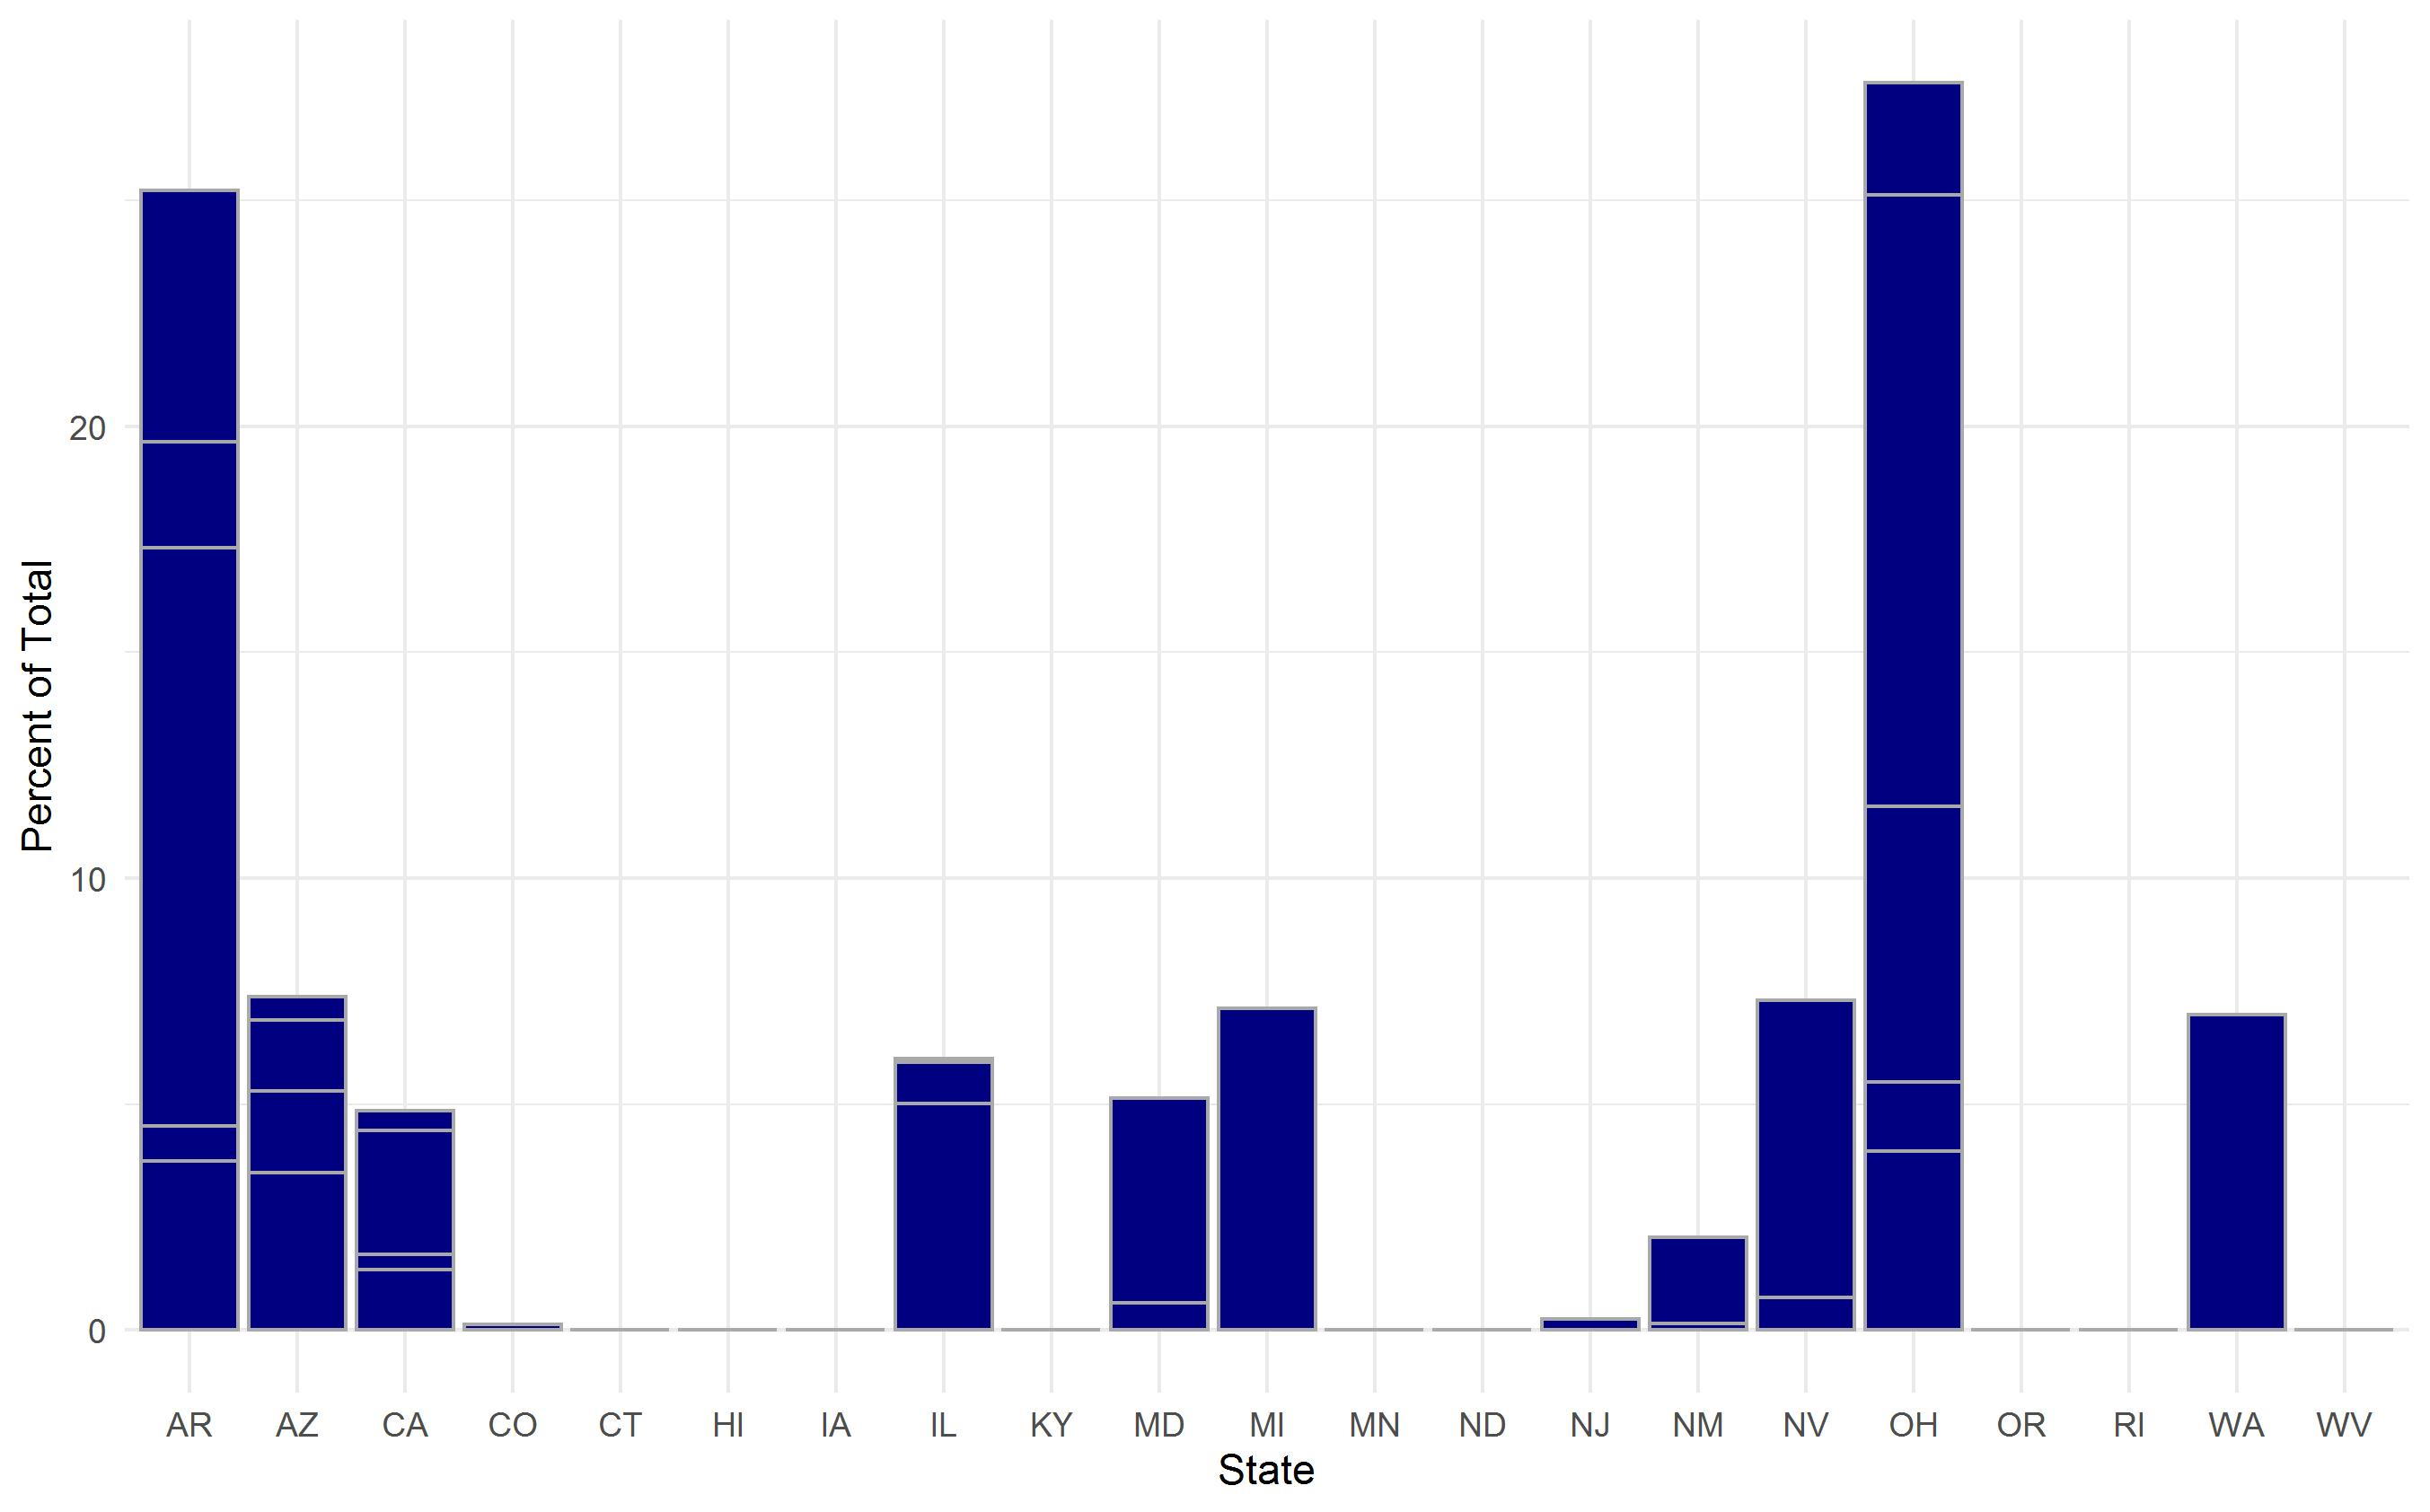
\includegraphics[scale=0.6]{cpuma-state-wgt-plot-new.png}
    \caption{CPUMA Weights by State}
\end{figure}

Using this weighting scheme we estimate a treatment effect of -2.21 (-1.32, -3.11). We also corrected for the remaining imbalances using a bias correction using linear regression; we found very similar estimates of -2.18 (-1.31, -3.06). We emphasize that these confidence intervals account for the randomness in the estimation error for the CPUMA-level outcomes and covariates and in the weighting procedure. These confidence intervals therefore implicitly condition on the particular randomization we saw, and account for the sampling variability of our CPUMA-level covariate estimates and the weighting procedure alone. This is in contrast to the types of ``placebo tests'' frequently seen in this literature that try to estimate the variance using the randomization distribution of treatment assignment (assumed to be uniform).

\begin{figure}
    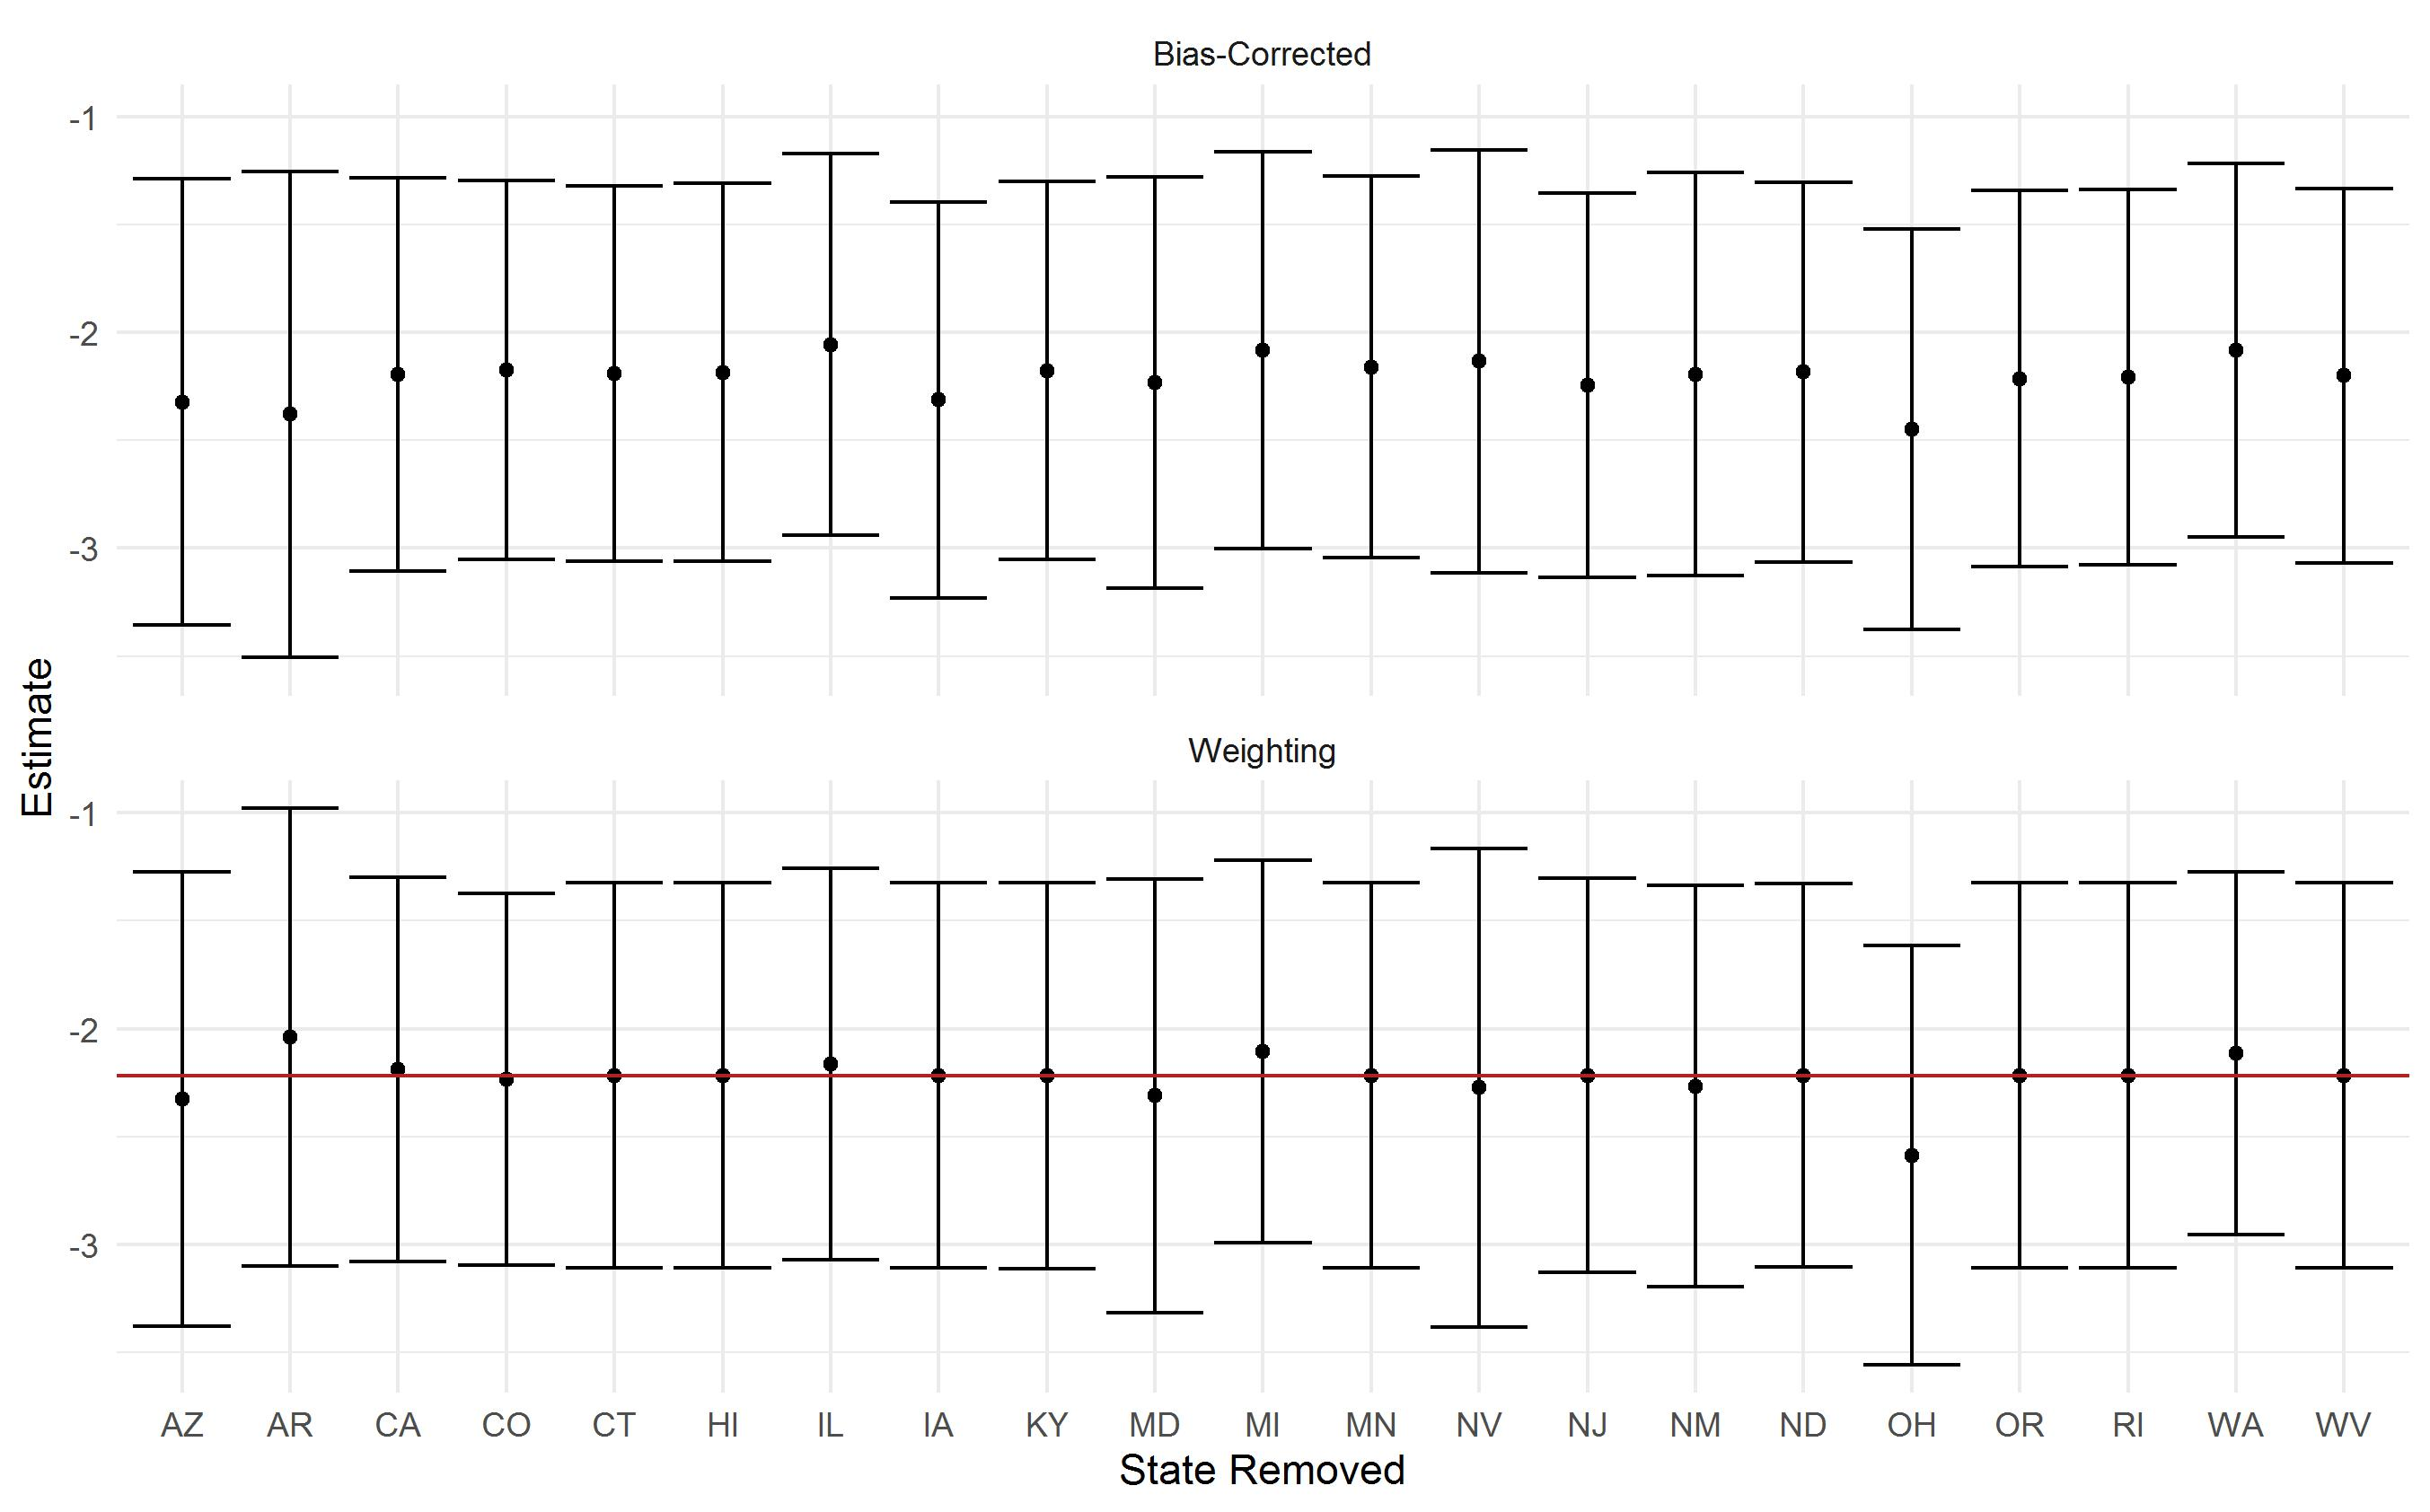
\includegraphics[scale=0.6]{loo-states-orig-dr.png}
    \caption{Leave-one-out state analysis}
\end{figure}

We examine how sensitive our estimates are to particular states. We therefore removed one state at a time and reran the procedure. Figure 4 presents the results for the weighting estimator and the bias-corrected estimator. Unsurprisingly, removing the states that received zero weights made no impact on our estimates. The results were somewhat sensitive to the exclusion of Arizona, Arkansas, and Ohio; in particular, the treatment effect moves further away from zero when we remove these states. Overall, we see that the results appear to be slightly less sensitive to the removeal of any particular state when when using the bias correction.

Our last analysis examines how important certain covariate groups are in determining these effects. We are especially interested how our treatment effects change when we remove the Republican governance indicators, since we hypothesize that this should be strongly associated with treatment effects closer to zero. We divide our covariates into six separate groups: pre-treatment uninsurance rates, pre-treatment unemployment rates, Republican governance indicators, racial demographics, education and poverty demographics, and other demographics (age, marital status, female, children). We then rerun the analyses excluding each group. Figure YY displays the results. We see that removing the Republican governance indicators results moves the treatment effect estimates further away from zero, while the results are less sensitive to the other groups (results were similar when the weighting-only estimator). 

\begin{figure}
    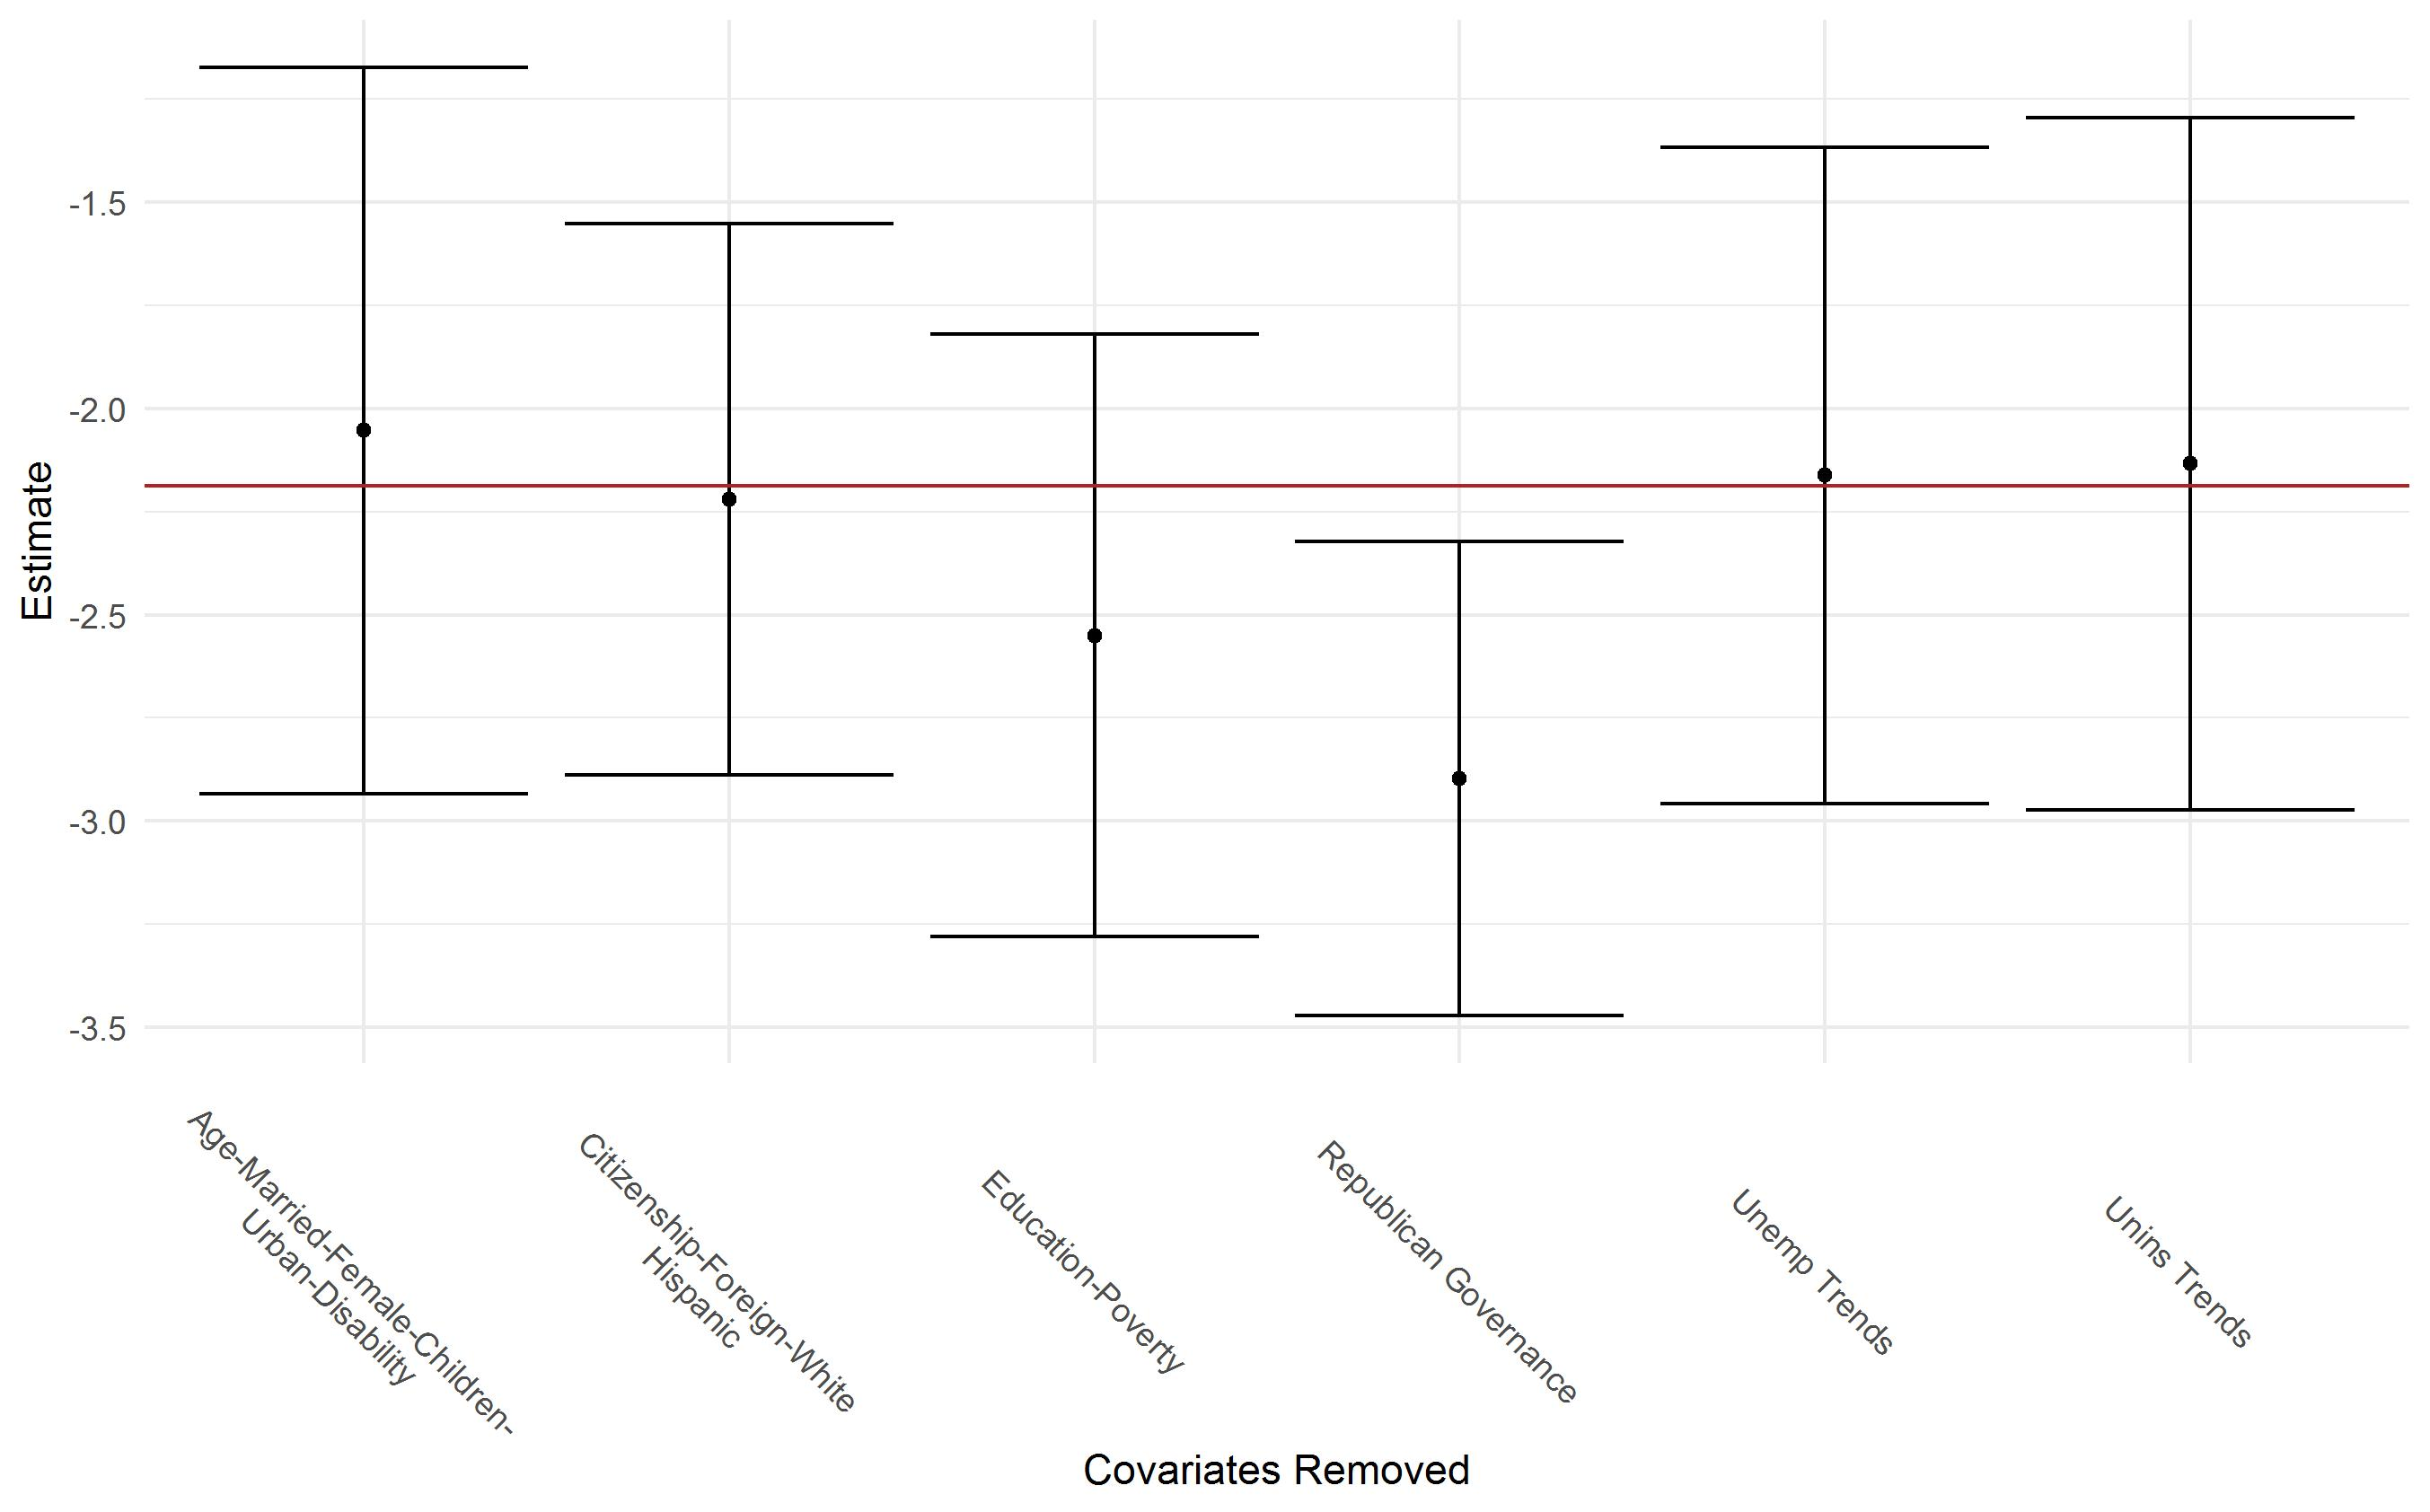
\includegraphics[scale=0.6]{loo-covariates-dr.png}
    \caption{Leave-one-out covariates}
\end{figure}

Overall these results suggest a strong relationship between the estimated treatment effect and Republican governance. However, Ohio and Arkansas are largely driving these estimates, and excluding these states may change this observed relationship. We therefore combined the leave-one-out covariate analysis with the leave-one-out state analysis to see how these estimated relationships changed. Figure XX presents the results for the Republican governance indicators alone. The blue bars and dot represents the estimated treatment effect when removing each state and the Republican governance indicators. The red dot represents the original leave-one-out-state estimates. We see that this negative association between Republican governance and the estimated treatment effect holds even when leaving particular states out. Results are similar for the weighting-only estimator. Full results for all covariate groups for both the bias corrected and weighting estimator are available in the Appendix.

\begin{figure}
    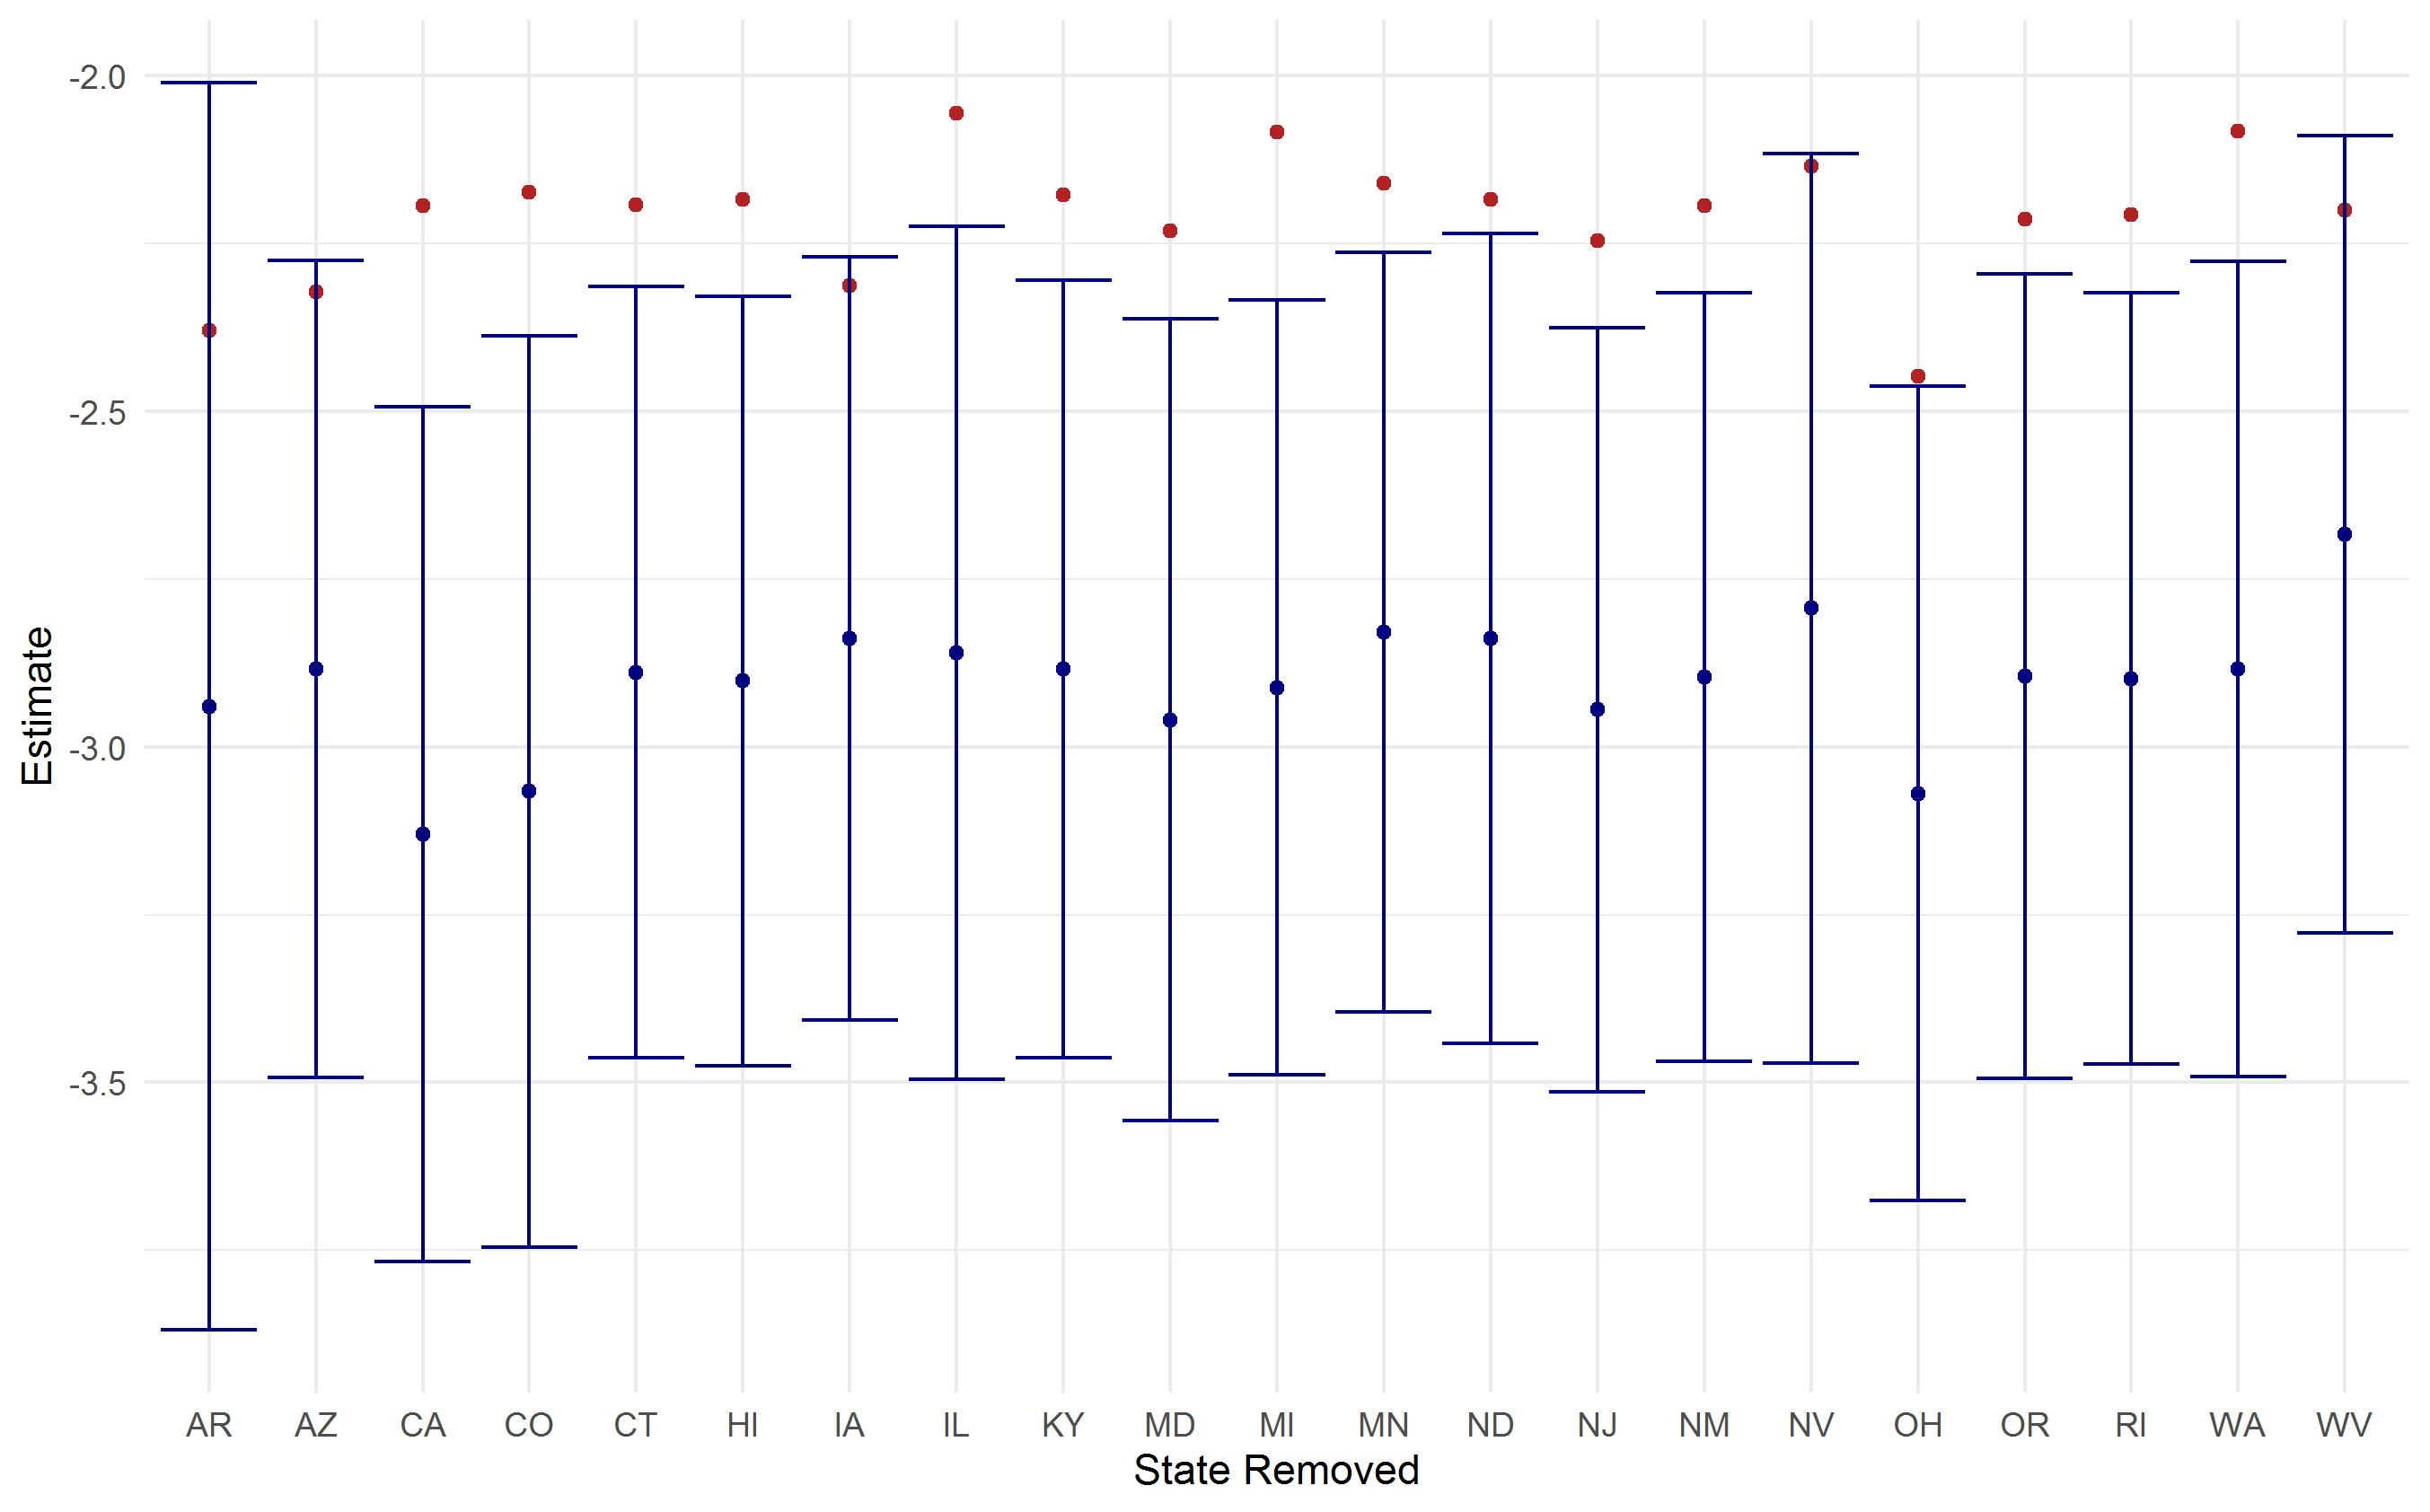
\includegraphics[scale=0.6]{loo-covs-state-repub-dr.png}
    \caption{Republican governance and leave-one-out state analysis}
\end{figure}

\subsection{Sensitivity Analyses}

In this section we examine the sensitivity of our results to violations of two key causal assumptions: (1) no anticipatory treatment effects, and (2) positivity violations.

As we noted early, several states had partial limited expansions prior to 2014. These states included California, Connecticut, Minnesota, New Jersey, and Washington. We rerun our analyses excluding CPUMAs from all five of these states. We are unsure how we should expect this to affect our estimates: on the one hand, states that expanded early might have a smaller treatment effect after 2014 because they already enrolled newly eligible individuals. This would bias our previously estimated treatment effect upwards. On the other hand, if these states were also more motivated to enroll people in Medicaid, they might have larger post-exapnsion coverage gains, leading to a downwards bias. When removing these states, we estimate an effect of -1.97 (-0.96, -2.98). This is consistent with the latter story. However, when we run the bias-corrected version we estimate -2.27 (-1.48, -3.38), which is consistent with the former. Regardless, the confidence intervals largely overlap. Overall these results suggest that the bias from potential anticipatory treatment effects from these states was negligible. Our leave-one-out covariate analysis shows similar results to those in our primary analysis (results available in the appendix).

Our final analysis tests the sensitivity of our estimates to positivity violations. Because we were not able to get full overlap, our weighting estimators suffer some bias due to the imbalances, and our bias-corrected estimators rely on linearly extrapolating from our data. We therefore target a different treatment effect here -- the overlap treatment effect, using overlap weights proposed by \cite{li2018balancing}. Using logistic regression, we generate weights that exactly balance the means of the covariates between control and treatment group. This is essentially a data-drive method to implement commonly used weight ``trimming'' procedures. The cost is that we now have a data-dependent treatment effect: the overlap average treatment effect, which represents the treatment effect within regions where there is covariate overlap. We therefore are changing the target parameter.

Figure 8 shows the the expansion state, non-expansion state, and overlap weight covariate means, ordered by the largest difference between expansion and non-expansion states. We see that the overlap region is in general closer to the non-expansion states. This is a more conservative, less diverse region. Interestingly, we also see that the pre-treatment uninsurance and unemployment rates are also lower than either the overall expansion or non-expansion states. In general we find that the average L2 distance between the expansion states and overlap region is 8.29 percentage points while it is only 2.91 between the non-expansion and overlap region. 

Figure 7 shows the total percentage contribution of CPUMAs within each state to the overall OATE weights by treatment group. Notice that many of the expansion states are heavily downweighted, whereas the distribution across the non-expansion states is more uniform. In particular, we see that Ohio and Michigan constitute over 50 percent of this regions weights, while the Pennsylvania, Wisconsin, Missouri, and Florida represent over 50 percent of the non-expansion state weights.

\begin{figure}
    \includegraphics[scale=0.6]{overlap-weights-state-weights-Preferred.png}
    \caption{OATE Percentage Weights by State}
\end{figure}


We estimate that the OATE is -2.02 (-1.63, -2.41). This result is virtually unchanged when we remove the potential early expansion states, giving an estimated effect of -2.01 (-1.61, -2.40). Figure 8 shows that results are quite insensitive to removing any particular non-expansion state, though they appear most sensitive to Ohio, Iowa, and Arkansas. Our leave-one-out covariate group again shows the negative association between Republican governance and the magnitude of the treatment effect. The leave-one-out covariate group by state analysis is available in the Appendix and is consistent with these results, again showing that Republican governance is negatively associated with the estimated treatment effect.

\begin{figure}
    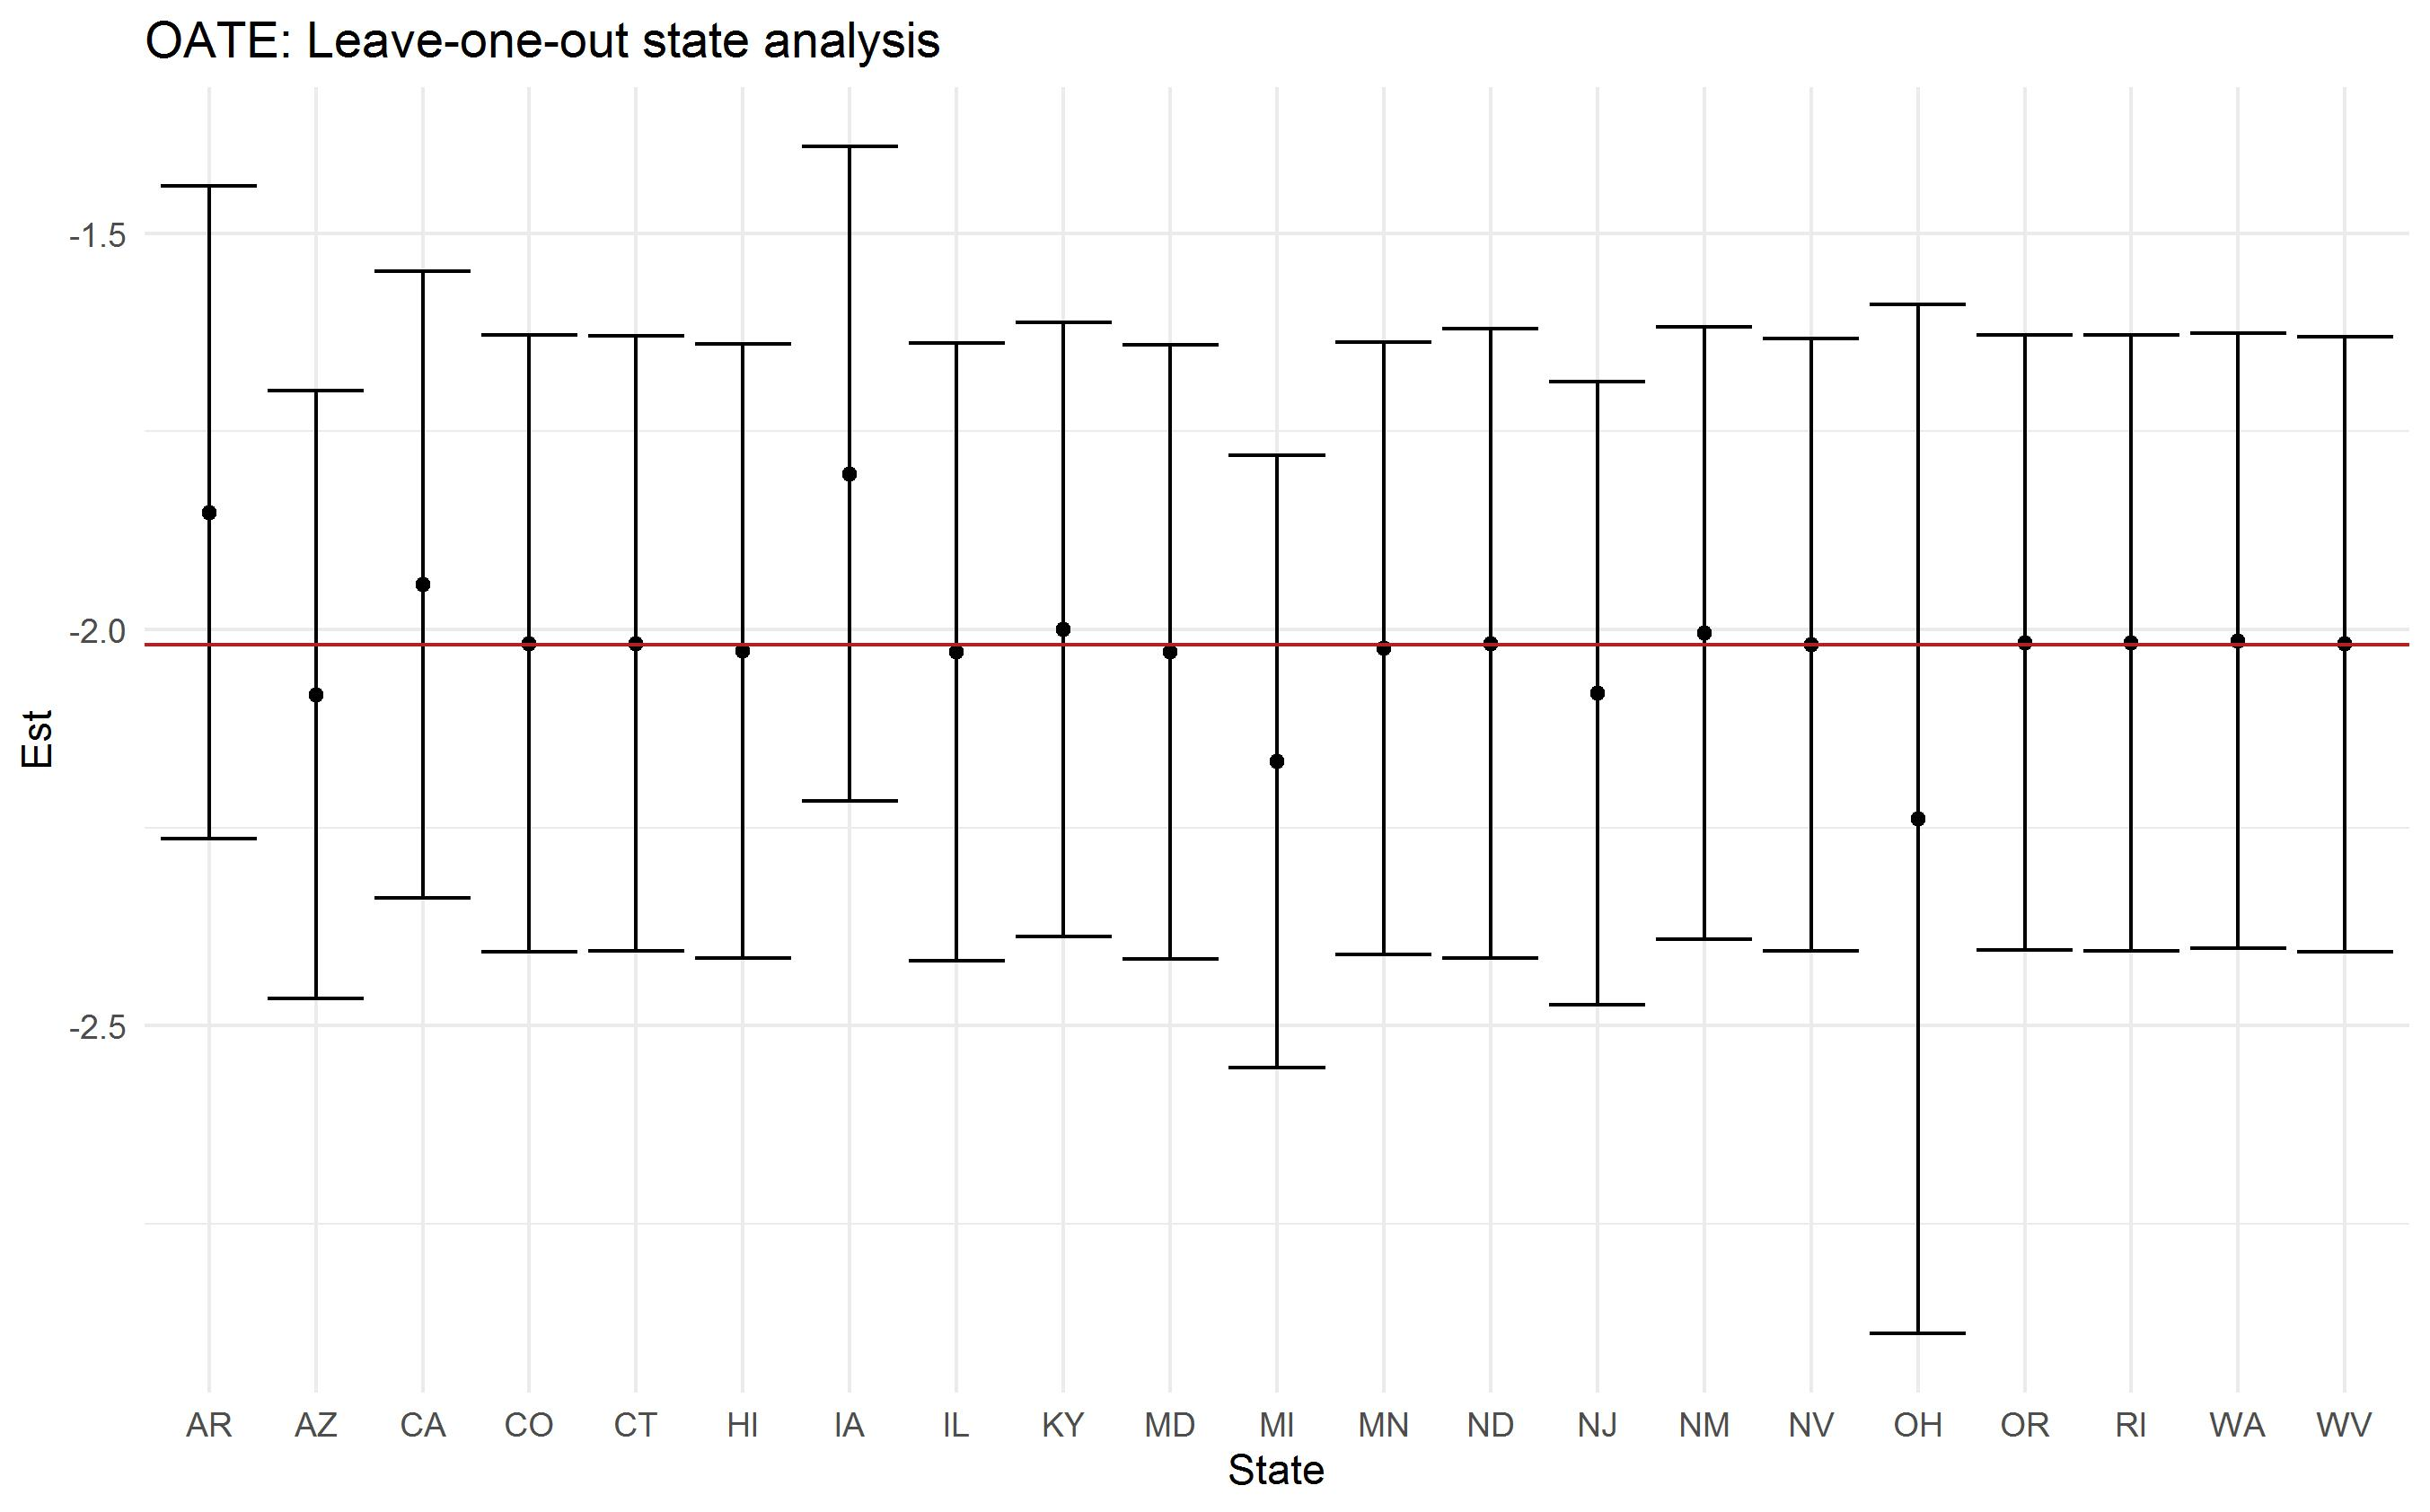
\includegraphics[scale=0.6]{oate-loo-state.png}
    \caption{OATE Leave-one-out state analysis}
\end{figure}

\section{Discussion}

This is the first study to directly estimate the ETU from Medicaid expansion. We estimate this effect is -2.18 (-1.31, -3.06). We also find a consistent negative association between the estimated treatment effect and Republican governance. 

These results have bearing on studies estimating the ETT using a differences-in-differences approach to study the 2014 effects of Medicaid expansion. In particular, the consistent negative association between Republican governance and the estimated treatment effect suggests that existing studies that fail to account for this effect modifier may incorrectly estimate the targeted treatment effects. The key point is that Medicaid expansion was implemented simultaneously with other aspects of the Affordable Care Act. In essence, the only possible counterfactual to implementing Medicaid expansion we can impute from the observed data is not implementing Medicaid expansion but implementing the other aspects of the Affordable Care Act. Letting $O$ representing the ACA, the ETT is more precisely denoted as:

$$
\mathbb{E}\{Y^{A = 1, O = 1} - Y^{A = 0, O = 1} | A = 1\}
$$

If we think then that the Republican governance is also associated with an attenuated effect of $O$ (many of these policies were implemented by the states), then using the observed change among non-expansion states to impute the counterfactual change among expansion states without controlling for governance may cause one to overestimate the treatment effect. Importantly, whether this is a concern depends on the particular outcome measure and how sensitive it is to effects from $O$. Because we use non-elderly adult uninsurance rates, this is a particular concern in our study, but may be less of a concern in others.

More generally, when we are concerned about the interactions between the treatment effect and governance, we find that there is likely insufficient overlap to account for these effects without extrapolating from the data. In fact, we find that the ETU requires less extrapolation than the ETT, as shown in our analysis targeting the OATE.

Our results are not without caveats: (1) We make strong parametric assumptions to identify our causal estimand. (2) We assume no unmeasured confounding; existing panel-data methods focus on estimating $Y^0$ given different parameterizations of unmeasured confounding, and we do not know of a better way to identify this effect in this setting. (3) We assume consistency at the CPUMA-level; it is likely that spillovers occurred not only across CPUMAs, but across states, which likely biases our estimates; and (4) our variance estimation only accounts for the uncertainty in the CPUMA-level measurements. In other words, if we knew the true covariates and outcome at the CPUMA-level, we would have no confidence intervals on our estimate; however, there are other sources of randomness we may wish to consider in that setting (in particular, randomness over the treatment assignment).

In summary, we use a weighting and bias-corrected estimators to estimate the effect of Medicaid Expansion on states that did not expand Medicaid in 2014. Regions from Ohio and Arkansa largely drive this initial result: however, we find that this result is largely insensitive to the exclusion of any particular expansion state. These estimates are also robust to sensitivity analyses examining potential violations of the assumptions of no anticipatory treatment effects and positivity violations. Moreover, we find evidence that Republican governance is associated with a treatment effect that is farther from zero. This association is also robust to the removal of each state and is consistent with evidence in the existing literature that finds that Medicaid take-up rates are lower in Republican-governed states \cite{sommers2012understanding}.


\cleardoublepage
\bibliography{research.bib} 

\cleardoublepage

\section{Appendix}

\subsection{Appendix A: SBW Program Details}

We implement SBW using the ``optweight'' package available in R. We use this program to generate weights that balance the means of the following covariates in the treated group to the control group within an error tolerance, $\delta$. These covariates include:

We $\delta$ to represent percentage point differences in the mean covariate values, and then convert this into absolute difference. In percentage points, we make the following error tolerances: $\delta = ()$.

When estimating the weights using the CPUMA-level datasets generated with the ACS replicate survey weights, $\delta^\star$ is not guaranteed to converge. We therefore modify the program so that if it does not converge, it relaxes some of the constraints until the program converges. In particular, we allow for the following relaxations that continue until convergence:

\subsection{Appendix B: Additional SBW Results}

Figure AA presents the results for the weighting estimator for the leave-one-out covariate group analysis (the paper only presents the bias corrected estimator).

\begin{figure}[H]
    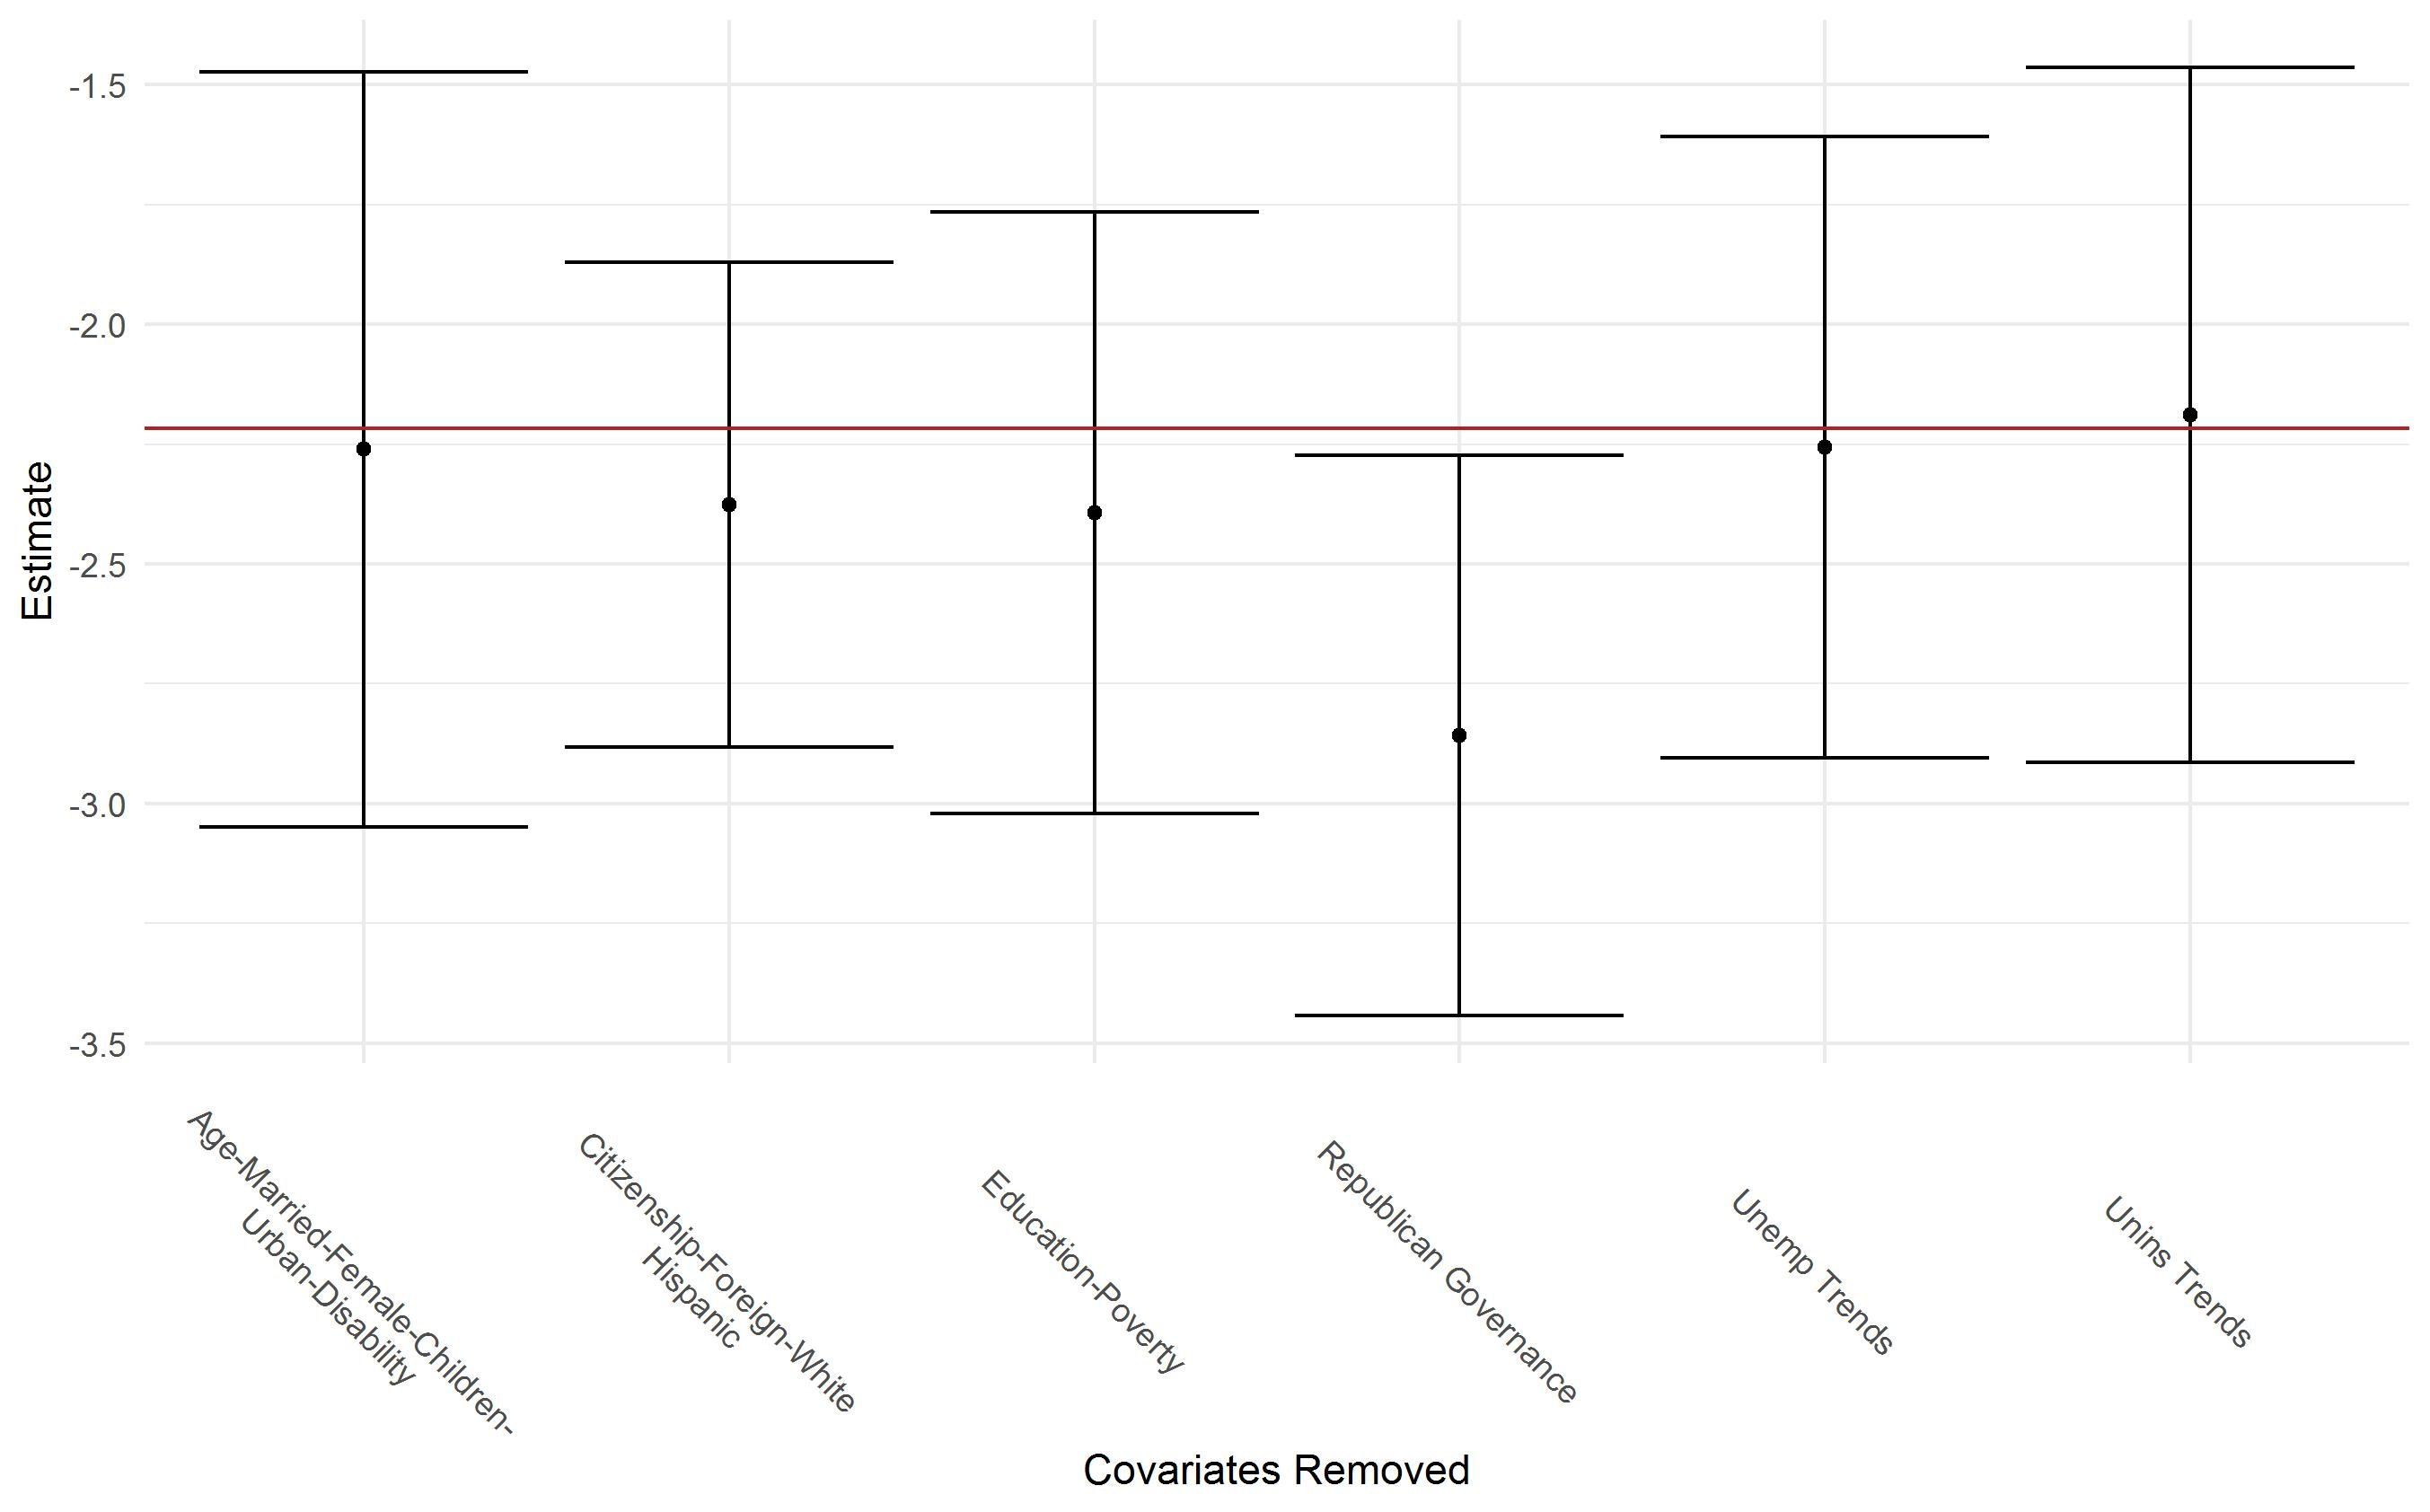
\includegraphics[scale=0.6]{loo-covariates-wgt.png}
    \caption{ETU Leave-one-out state analysis: weighting estimator}
\end{figure}


Figures ZZ and YY below presents the associations between each covariate group and the estimated treatment effect when removing each non-expansion state one at a time. The red horizontal lines represent the estimated ETU for each set of states. The top figure presents results for the weighting estimator and the bottom figure for the bias-corrected estimator. We again see that Republican governance is negatively associated with the estimated treatment effect throughout.

\begin{figure}[H]
    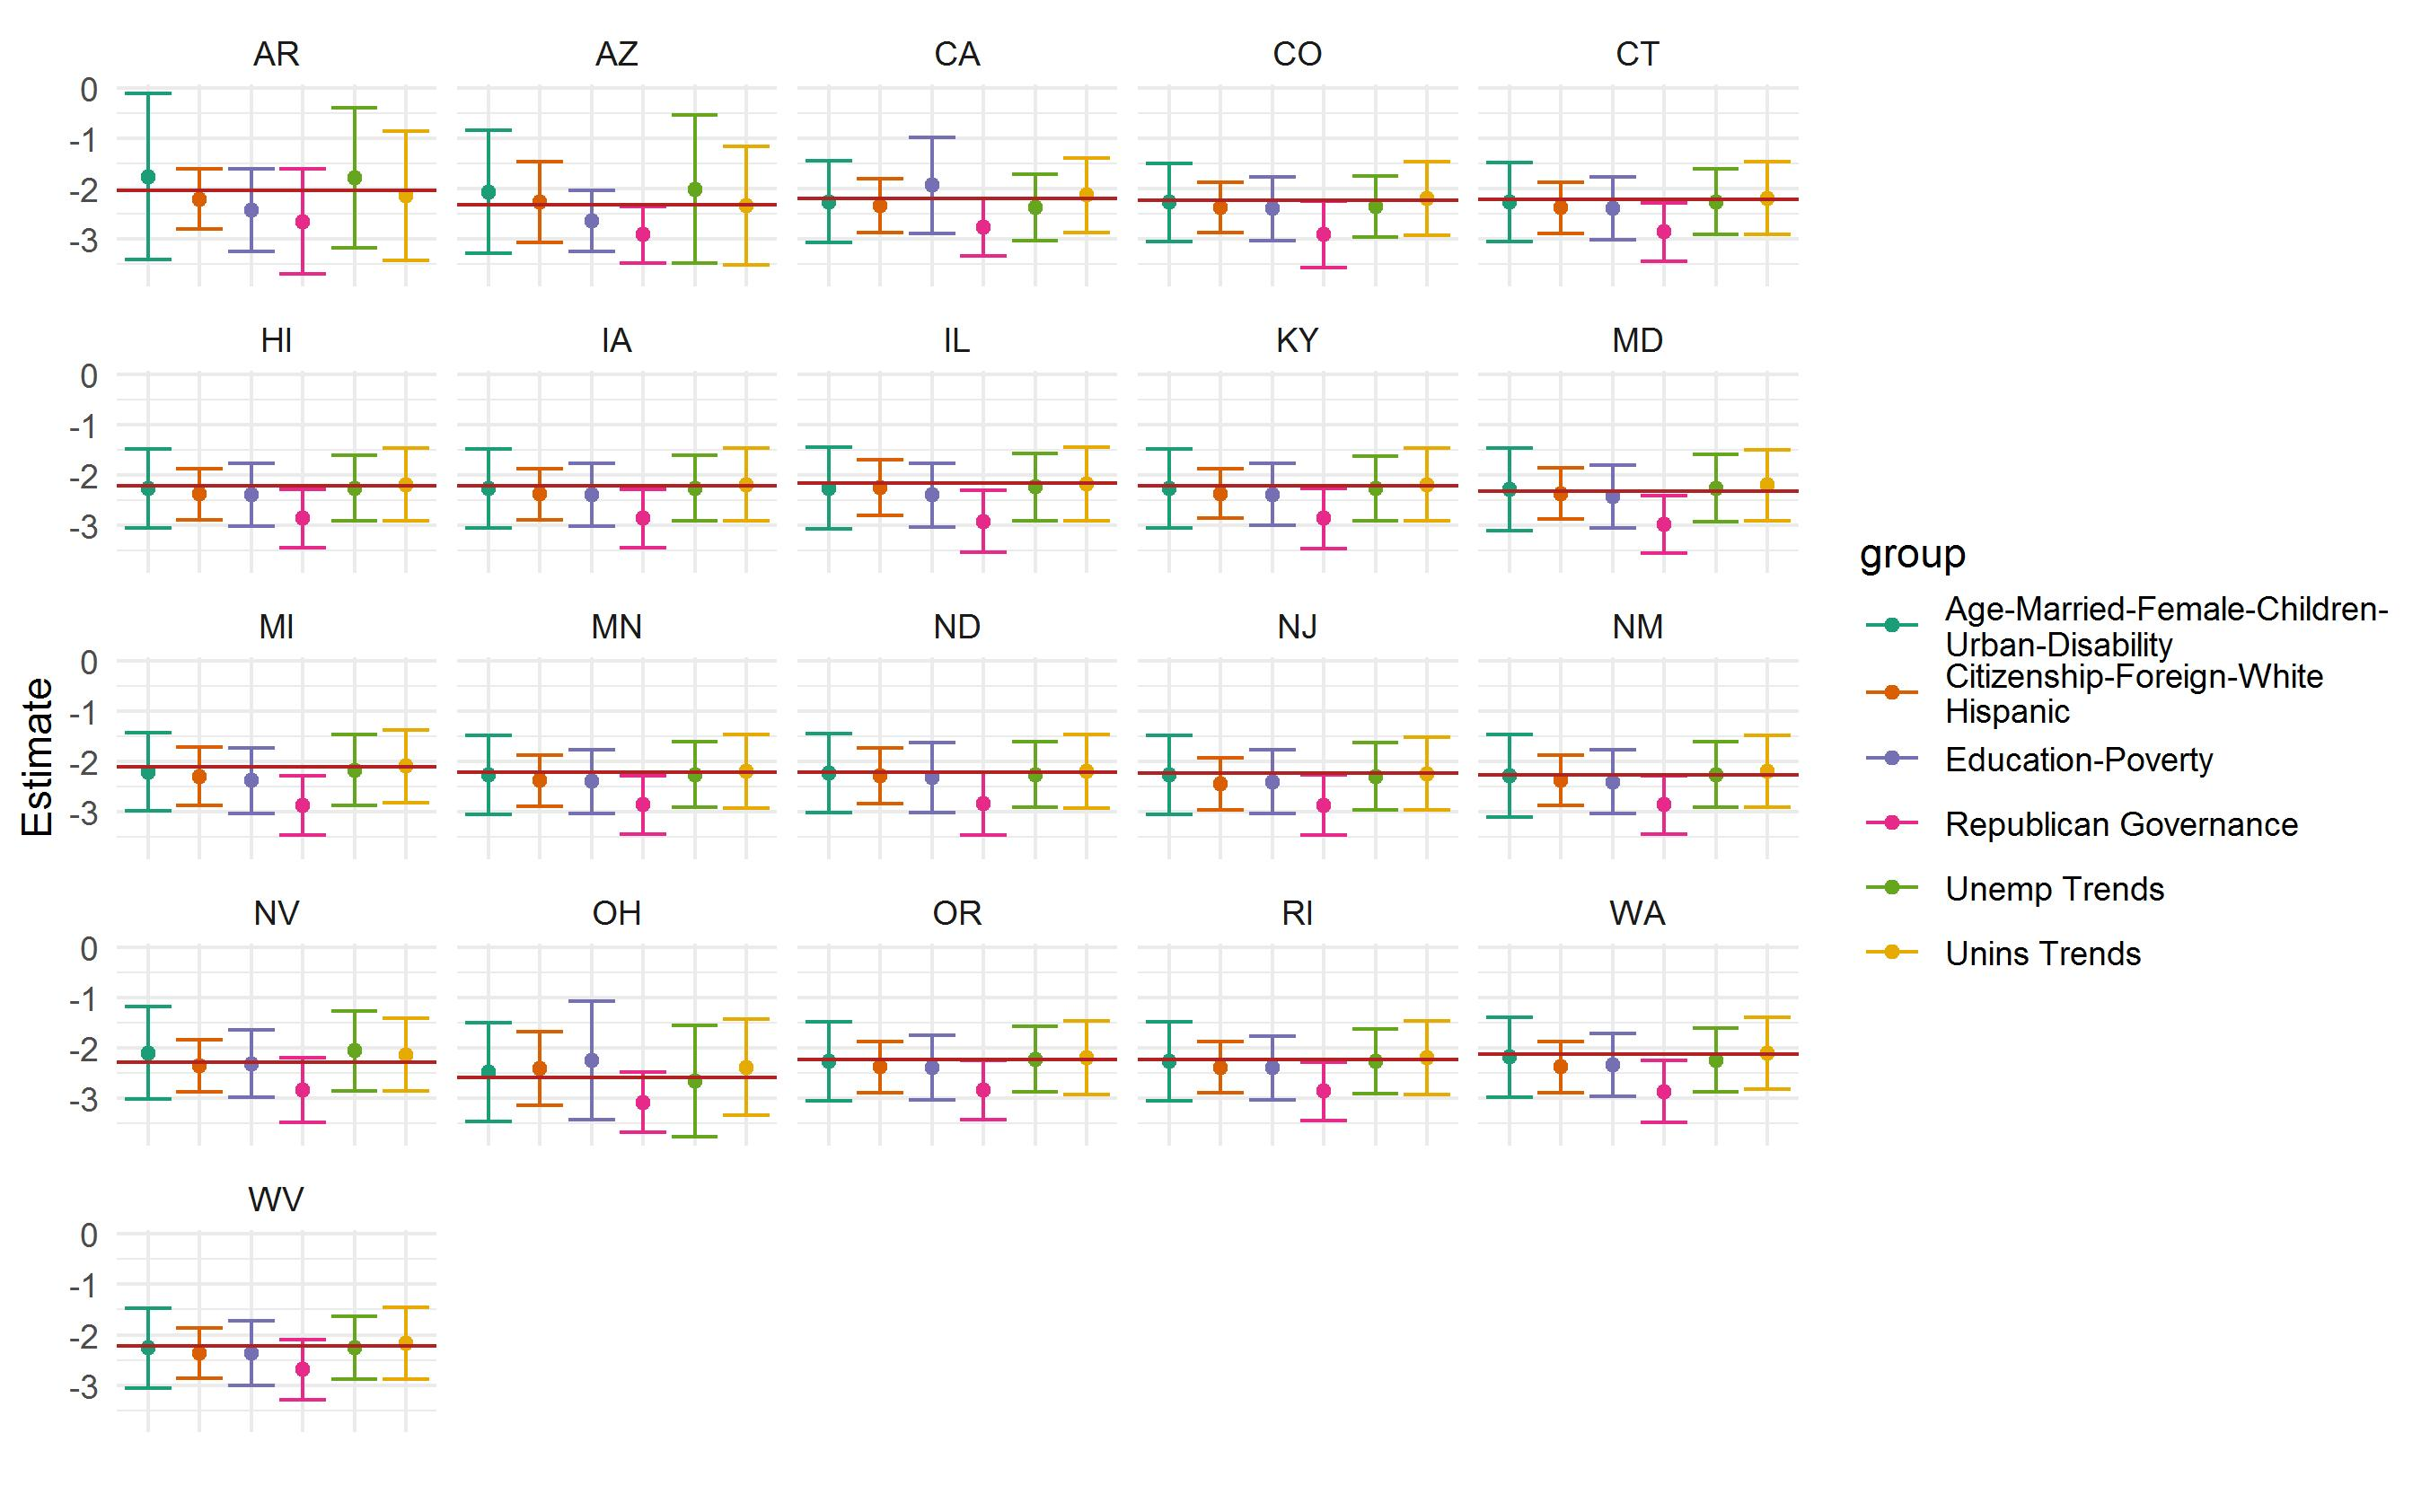
\includegraphics[scale=0.6]{loo-covs-state-all-wgt.png}
    \caption{ETU Leave-one-out states and covariates analysis: weighting estimator}
\end{figure}

\begin{figure}[H]
    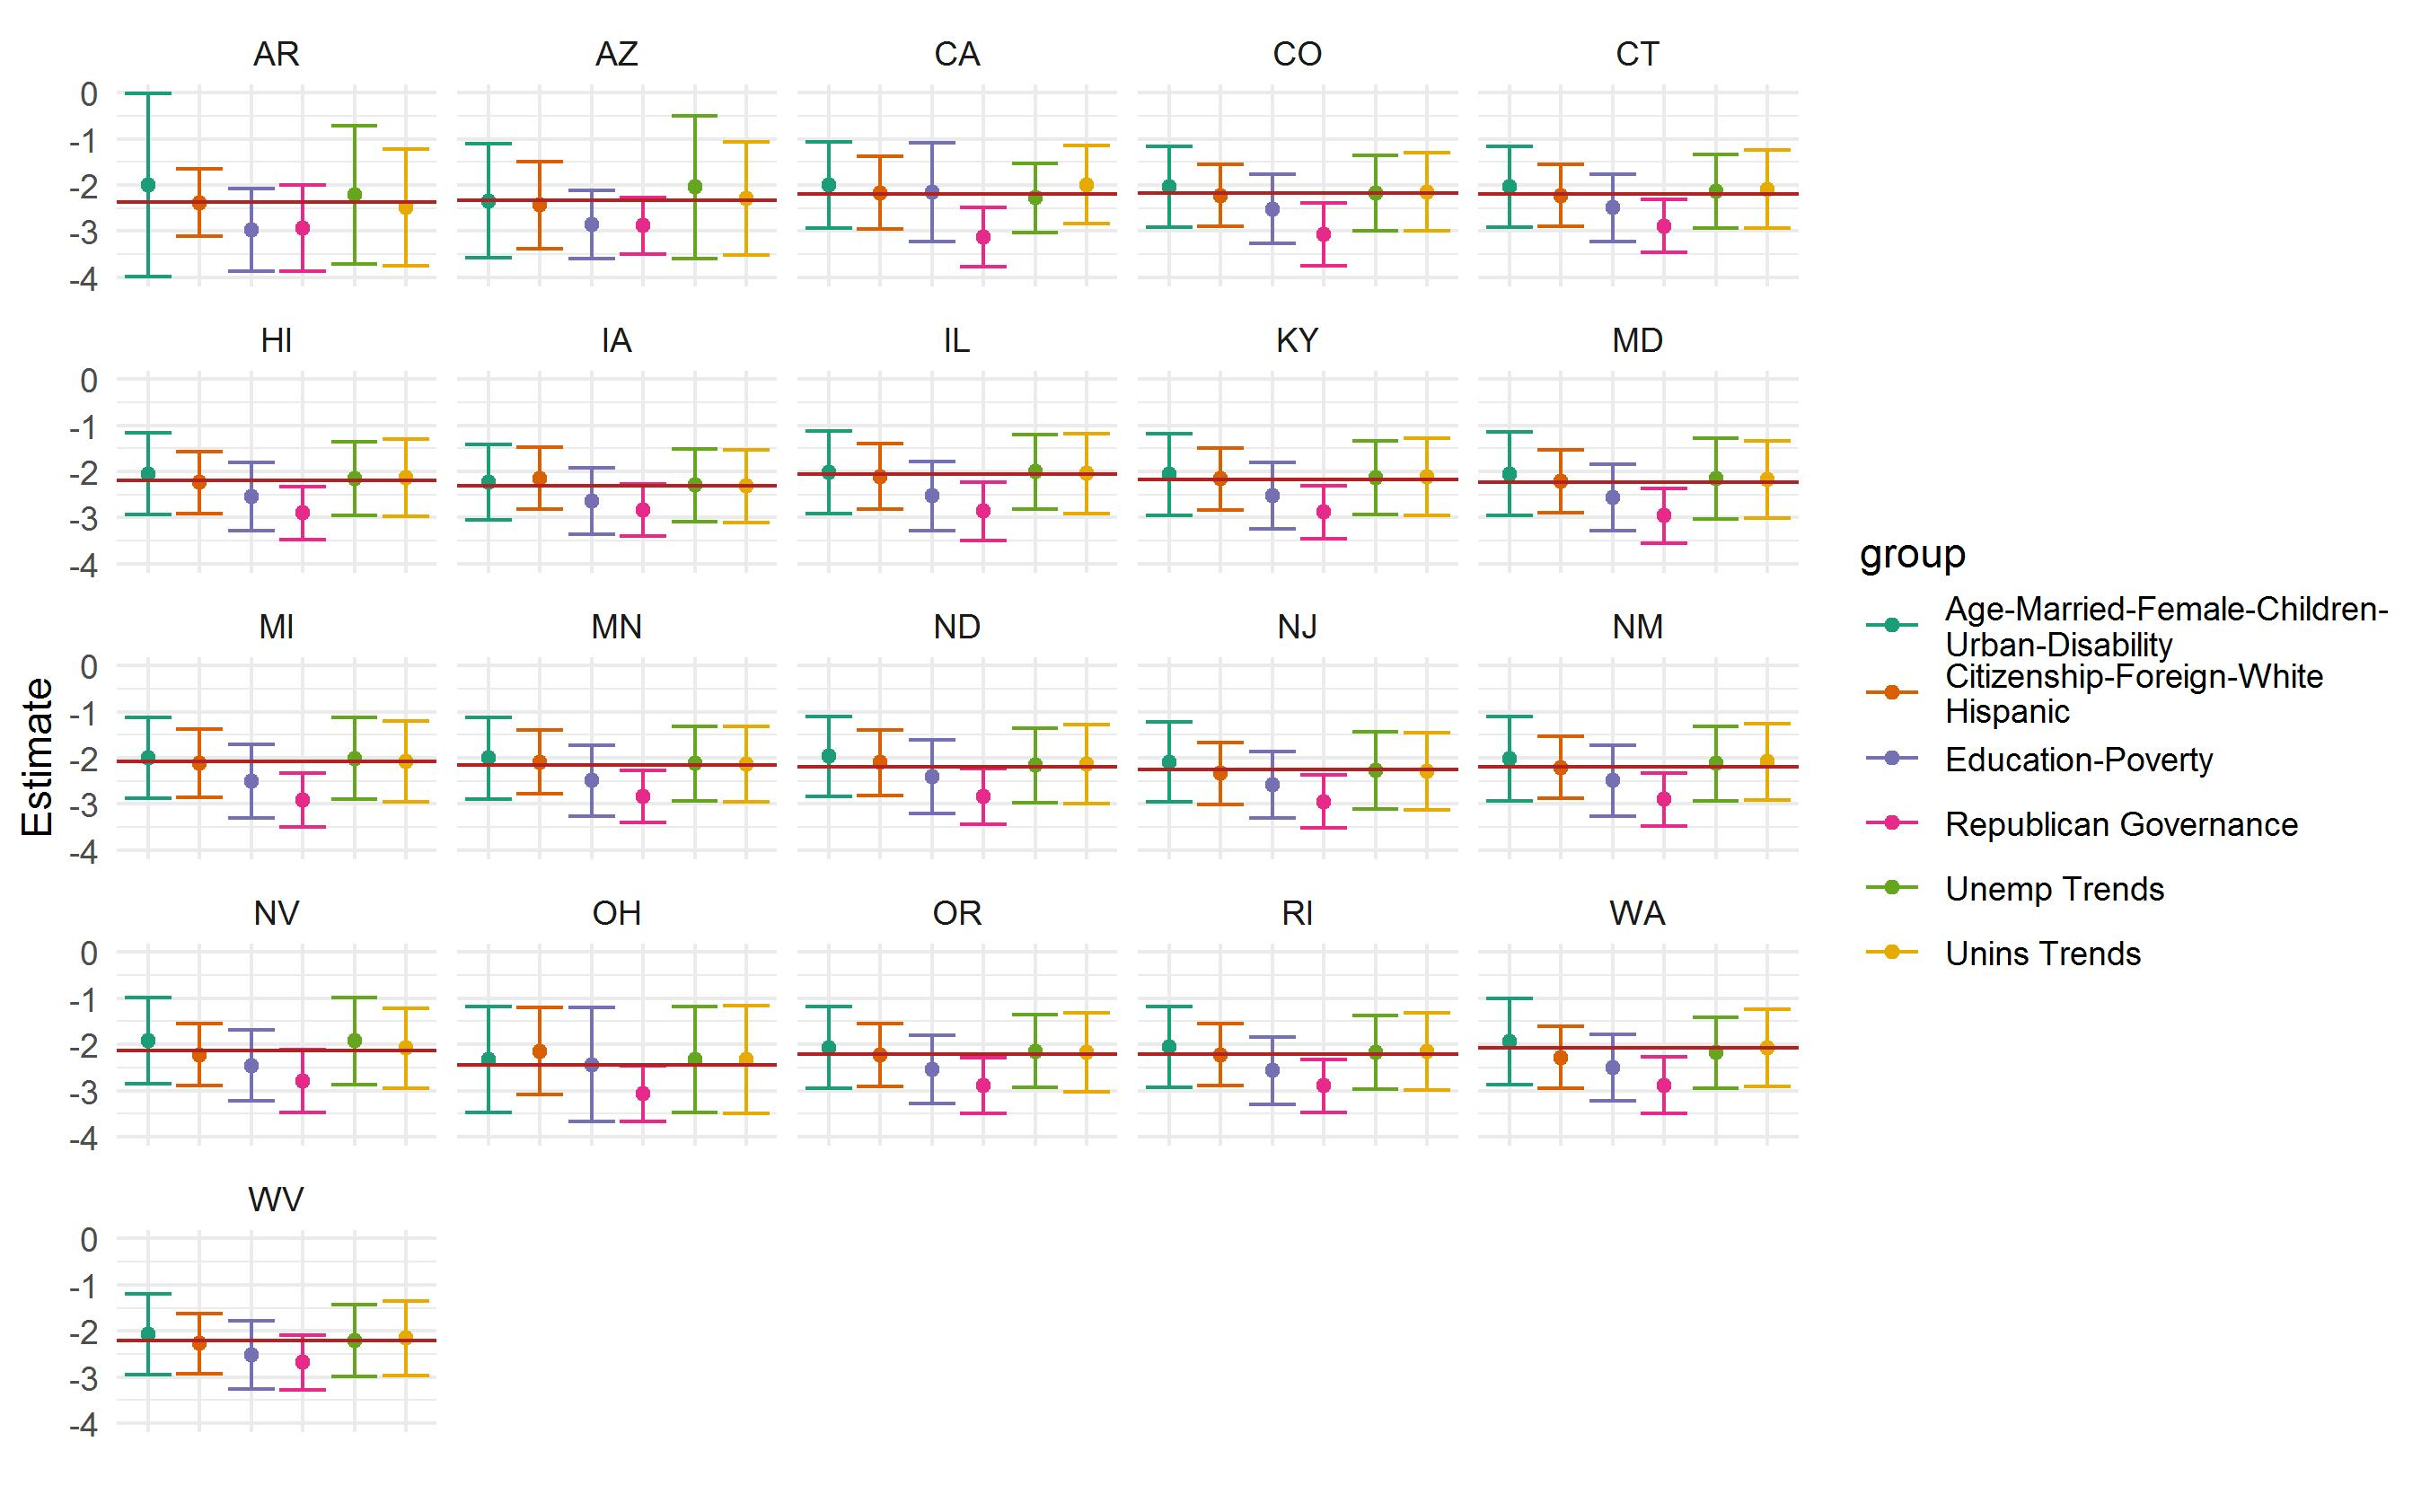
\includegraphics[scale=0.6]{loo-covs-state-all-dr.png}
    \caption{ETU Leave-one-out states and covariates analysis: bias-corrected estimator}
\end{figure}


\subsection{Appendix C: Additional OATE Results}

Figure ZZ below presents the associations between each covariate group and the estimated treatment effect when removing each non-expansion state one at a time. The red horizontal lines represent the estimated OATE for each set of states. We again see that Republican governance is negatively associated with the estimated treatment effect throughout.

\begin{figure}[H]
    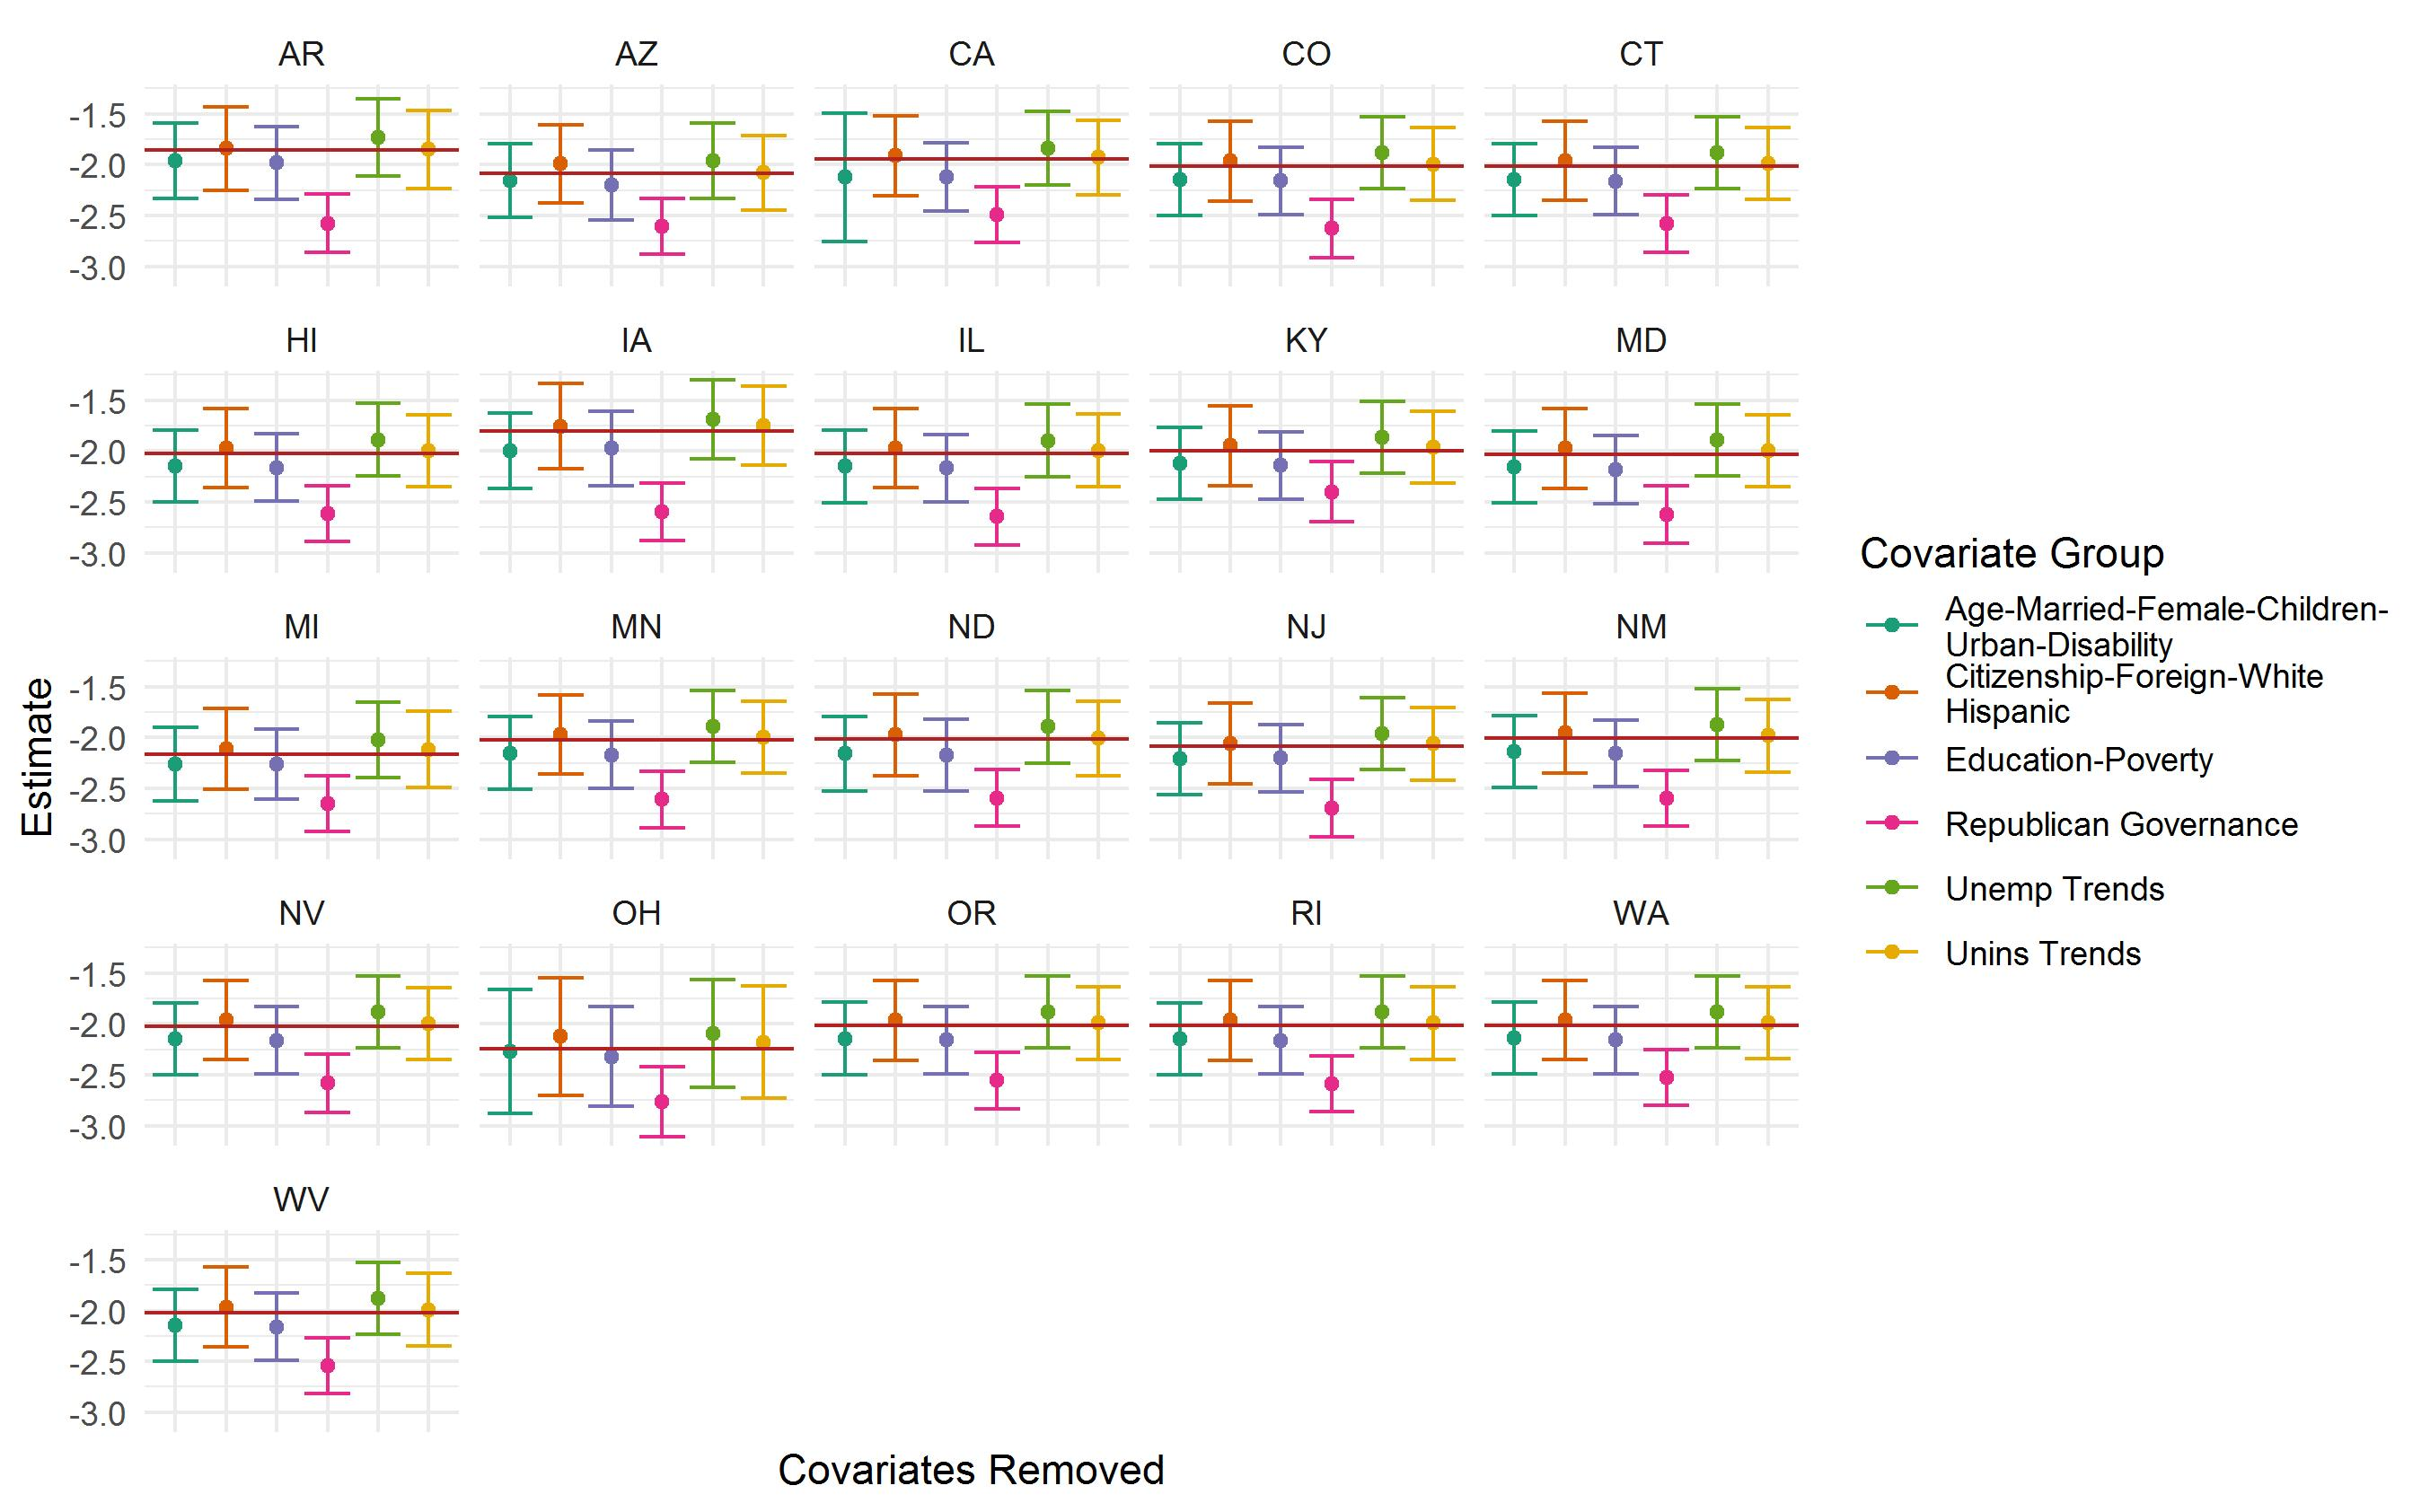
\includegraphics[scale=0.6]{oate-loo-covs-states.png}
    \caption{OATE Leave-one-out state analysis}
\end{figure}

\end{document}






